\documentclass[10pt, xcolor={usenames, dvipsnames}]{beamer}
%\documentclass[handout, 10pt, xcolor={usenames, dvipsnames}]{beamer}

\usepackage{etex}
\usepackage[french]{babel}
\usepackage[utf8]{inputenc}
\usepackage[T1]{fontenc}
\usepackage{amsfonts}
\usepackage{amsmath}
\usepackage{amssymb}
\usepackage{graphicx}
\usepackage{hyperref}
\usepackage{booktabs}
\usepackage[round]{natbib}
\usepackage{tikz}
\usepackage{colortbl}
\usepackage{ulem}
\usepackage{multicol}
\usepackage[overlay]{textpos}
\usepackage{multirow}
\usepackage{ragged2e}
\usepackage{rotating}
\usepackage{fancybox}
\usepackage{ulem}
\usepackage{overpic}
\usepackage{enumerate}
\usepackage{xfrac}
\usepackage{pgfplots}

\usepackage{epstopdf}
\usepackage{epsfig}

\setcounter{tocdepth}{2}

 \usetheme[style=termith]{min}

\pgfplotsset{compat=1.8}
\usetikzlibrary{positioning, topaths, shapes, arrows, patterns, calc}
\tikzstyle{io}=[
  ellipse,
  minimum width=5cm,
  minimum height=2cm,
  fill=termithgreen!30,
  draw=termithgreen!40,
  transform shape,
  font={\huge}
]
\tikzstyle{selectedio}=[
  io,
  fill=termithorange!30,
  draw=termithorange!40,
]
\tikzstyle{component}=[
  thick,
  rectangle,
  minimum width=13cm,
  minimum height=2cm,
  text centered,
  text width=12.5cm,
  fill=Cerulean!20,
  draw=Cerulean!30,
  transform shape,
  font={\huge\bfseries}
]
\tikzstyle{selectedcomponent}=[
  component,
  fill=termithorange!30,
  draw=termithorange!40,
]

\title{Édition collaborative dans les navigateurs}
\author{Brice \textsc{N\'edelec}}
\institute{\normalsize{Université de Nantes, LINA}}
\date{Thèse de doctorat soutenue le\\5 Octobre 2015}
\titlepageextra{
  \textbf{\large Jury}
  \\~\\
  \begin{tabular}{ll}
    \textbf{Président~:} & \textbf{Marc \textsc{Gelgon}}, Professeur des universités, Université de Nantes\\
    \textbf{Rapporteurs~:} & \textbf{Anne-Marie \textsc{Kermarrec}}, Professeur des universités, INRIA\\
                         & \textbf{Peter \textsc{Van Roy}}, Professeur des universités, Université de Louvain\\
    \textbf{Examinateurs~:} & \textbf{G\'erald \textsc{Oster}}, Maître de conférences, Université de Lorraine\\
                         & \textbf{Marc \textsc{Shapiro}}, Professeur des universités, INRIA \\
    \textbf{Directeur~:} & \textbf{Pascal \textsc{Molli}}, Professeur des universités, Université de Nantes\\
    \textbf{Co-directeur~:} & \textbf{Achour \textsc{Most\'efaoui}}, Professeur des universités, Université de Nantes\\
  \end{tabular}
}
\logos{
  \hfill{}\includegraphics[height=2em]{logos/LINA.eps}
  \hfill{}
\includegraphics[height=2em]{logos/UniversiteNantes.eps}
  \hfill{}
\includegraphics[height=2em]{logos/UBL.pdf}
  \hfill{}
}


\begin{document}

  \begin{frame}[plain, noframenumbering]
    \titlepage
  \end{frame}

  \section{Introduction}


% \begin{frame}{Introduction}\framesubtitle{Édition collaborative}

%   L'édition collaborative concerne toutes les activités effectuées en
%   \textbf{groupe} dans le but de produire un \textbf{document}. L'effort
%   collectif permet de bénéficier de multiples points de vues différents.

%   \begin{itemize}
%   \item[$\rightarrow$] Les documents sont de \textbf{meilleure qualité}.
%   \end{itemize}
  
%   \vspace{1cm}

%   \begin{minipage}{0.6\textwidth}
%     \textit{La version anglaise de Wikipédia compte \textbf{5 millions}
%       d'articles, \textbf{40 millions} de pages et \textbf{112 mille}
%       utilisateurs actifs.\vspace{0.15cm}\\Les articles possèdent une
%       \textbf{fiabilité} \textbf{comparable} à celle de l'Encyclopædia
%       Britannica.}
%   \end{minipage}\footfullcite{giles2005internet}
%   \hfill
%   \begin{minipage}{0.3\textwidth}
%     \begin{figure}
%       \begin{center}
%         
\includegraphics[width=0.7\textwidth]{img/wikipedia.png}
%       \end{center}
%     \end{figure}
%   \end{minipage}

% \end{frame}


\begin{frame}{Introduction}{Éditeur collaboratif}
%  \begin{minipage}{0.53\textwidth}
%     Un éditeur collaboratif permet
%     \begin{itemize}
%     \item à \textbf{plusieurs personnes}
%     \item de \textbf{lire} et \textbf{modifier} un document.
%       % \begin{itemize}
%       % \item \textbf{ajout} de caractères
%       % \item \textbf{suppression} de caractères
%       % \end{itemize}
%     \end{itemize}
    
%     Grâce au Web,
%     \begin{itemize}
%     \item n'importe quel outil accédant à l'internet (\textit{e.g. ordinateur,
%         smartphone, tablette}) permet de créer et d'éditer un document aisément.
%     \item Un simple lien permet de le partager facilement avec des amis ou des
%       collègues.
%     \end{itemize}    
% %  \end{minipage}
% %  \begin{minipage}{0.45\textwidth}
%     \begin{figure}    
%       \begin{center}
%         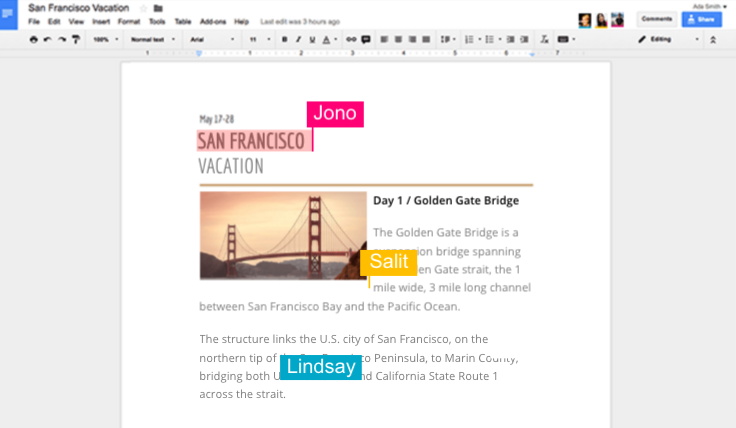
\includegraphics[width=0.65\textwidth]{img/googledocs.png}
% %        \caption{Capture d'écran d'un document Google Docs rédigé par 3 personnes
% %          en simultané. \REF}
%       \end{center}
%     \end{figure}
%  \end{minipage}
  
  \begin{textblock*}{\textwidth}(-1cm,-3cm) 
    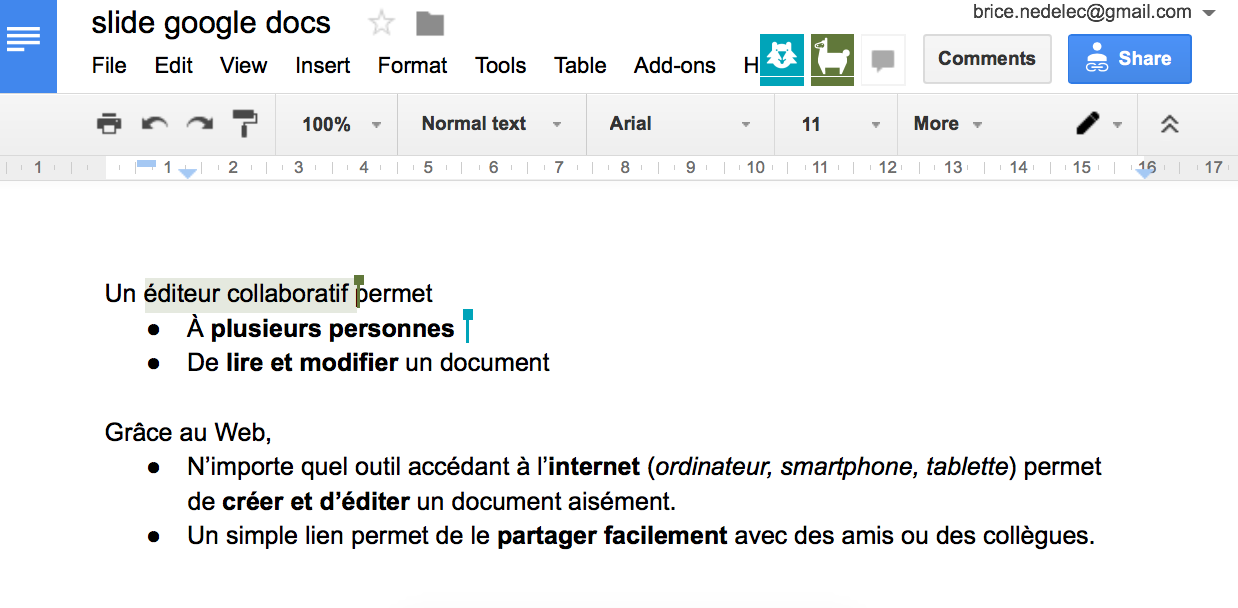
\includegraphics[width=1.19\textwidth]{img/googledocs3.png}
    % \footfullcite{johansen1988groupware}
%    \vspace{0.25cm}
  \end{textblock*}

%   \begin{textblock*}{\textwidth}(0cm,3cm)
% %    \large
%     \begin{itemize}
%     \item [$\Rightarrow$] Besoin ancien~\footfullcite{engelbart1968research};
%     \item [$\Rightarrow$] Mais une adoption récente : l'édition \textbf{temps
%         réel} et le \textbf{Web} contribuent grandement à leur popularité.
%     \end{itemize}    
%   \end{textblock*}
  
%   \vspace{0.25cm}
  
\end{frame}


\begin{frame}{Introduction}{Problèmes de centralisation}
  
%  \hspace{-1cm}
  Problèmes de \textbf{confidentialité}, \textbf{censure},
  \textbf{intelligence économique}, \textbf{legislation}, etc.

  \vspace{0.5cm}
  \begin{center}
    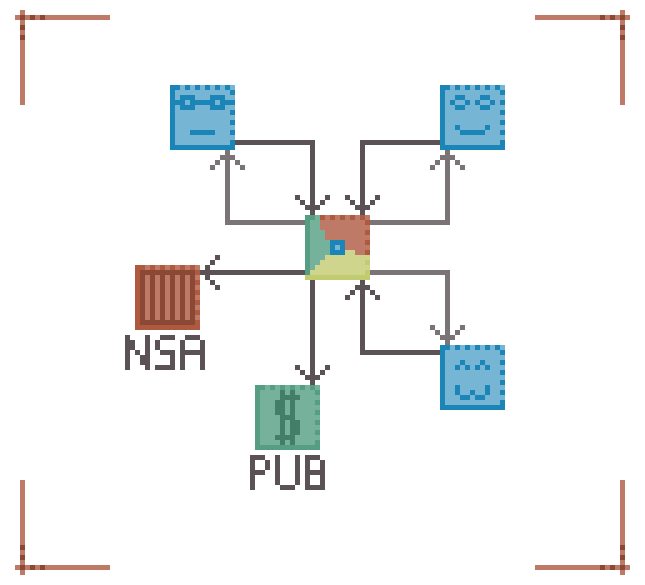
\includegraphics[width=0.5\textwidth]{img/centralizedethicproblems.png}
  \end{center}
  
  \vspace{0.5cm}

  \textit{En 2013, les révélations sur PRISM montre que la NSA possède des
    accès aux données hébergées par Google, Facebook, YouTube, Microsoft,
    Yahoo!, Skype, AOL et Apple.}

\end{frame}

\begin{frame}{Introduction}{Problèmes de centralisation}
  
%  \hspace{-1cm}
  % \begin{minipage}{0.69\textwidth}
  %   Problèmes de \textbf{confidentialité}, \textbf{censure},
  %   \textbf{intelligence économique}, \textbf{legislation}, etc. \vspace{0.15cm}\\
  %   \small\textit{En 2013, les révélations sur PRISM montre que la NSA possède des
  %     accès aux données hébergées par Google, Facebook, YouTube, Microsoft,
  %     Yahoo!, Skype, AOL et Apple.}
  % \end{minipage}
  % \hfill
  % \begin{minipage}{0.3\textwidth}
  %   \hfill
  %   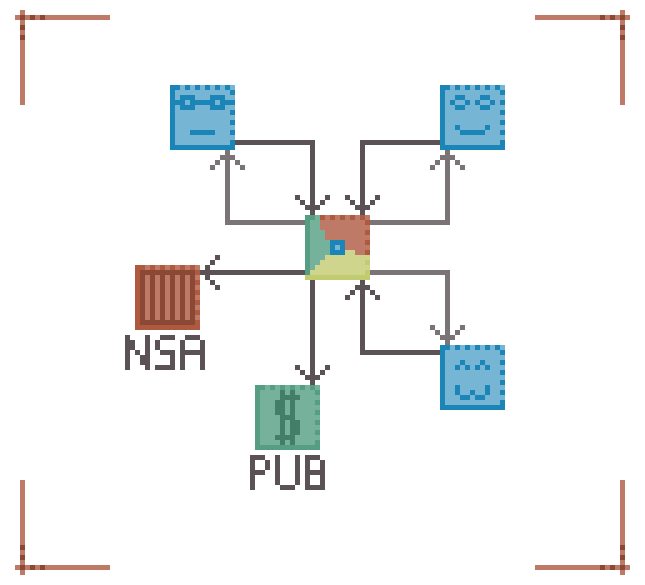
\includegraphics[width=0.97\textwidth]{img/centralizedethicproblems.png}
  % \end{minipage}

  Problèmes de passage à l'échelle, notamment en \textbf{nombre de
    collaborateurs}.
  
  \vspace{0.5cm}
  
  \begin{center}
    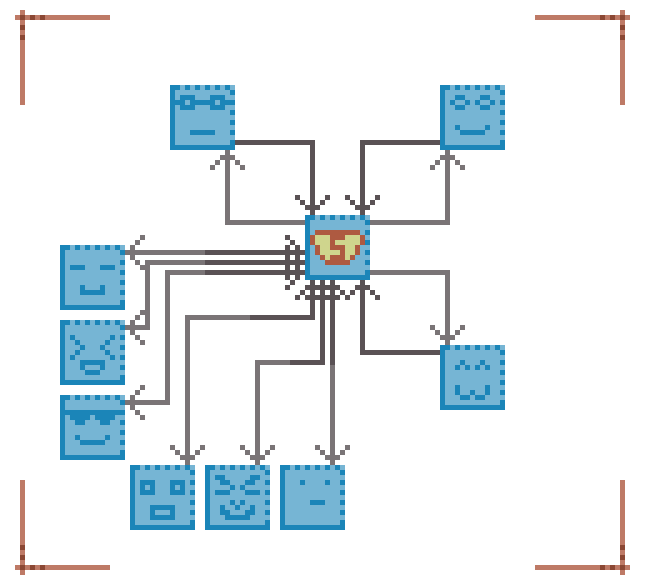
\includegraphics[width=0.5\textwidth]{img/centralizedcpuproblems.png}
  \end{center}
  
  \vspace{0.25cm}

  \textit{En 2013, Coursera rassembla 41000 étudiants sur un seul cours.  Les
    limitations de l'outil collaboratif utilisé conduisirent au \og
    désastre\fg\footfullcite{strauss2013how}.}

  \vspace{0.25cm}

  % \begin{minipage}{0.69\textwidth}
  %   Problèmes de passage à l'échelle, notamment en \textbf{nombre de
  %     collaborateurs}. \vspace{0.15cm}\\
  %   \small\textit{En 2013, Coursera rassembla 41000 étudiants sur un seul cours.  Les
  %     limitations de l'outil collaboratif utilisé conduisirent au \og
  %     désastre\fg.}% \footfullcite{strauss2013how}.}
  % \end{minipage}
  % \hfill
  % \begin{minipage}{0.3\textwidth}
  %   \hfill
  %   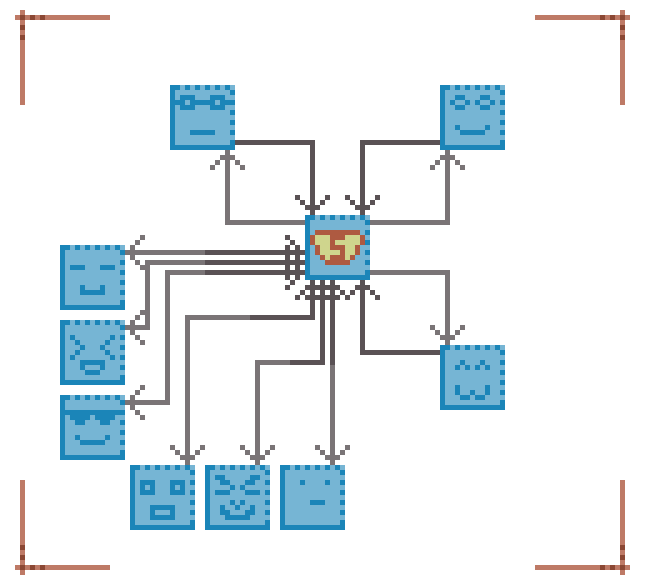
\includegraphics[width=0.97\textwidth]{img/centralizedcpuproblems.png}
  % \end{minipage}


  % \begin{minipage}{0.69\textwidth}
  %   Problèmes de \textbf{robustesse face aux défaillances}.
  % \end{minipage}
  % \hfill
  % \begin{minipage}{0.3\textwidth}
  %   \hfill
  %   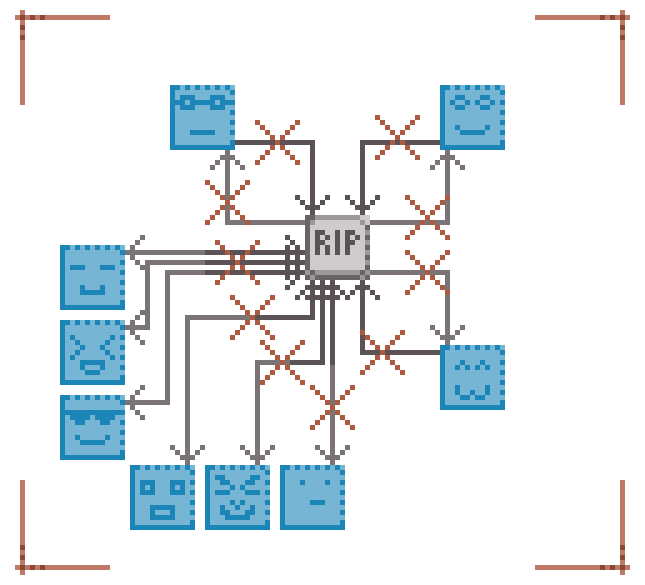
\includegraphics[width=0.97\textwidth]{img/centralizedscalabilityproblems.png}
  % \end{minipage}

\end{frame}


\begin{frame}{Introduction}{Ce que l'on veut : un éditeur collaboratif \ldots}
  
%  \begin{textblock*}
  \begin{minipage}{0.45\textwidth}
    \hfill \YES{\cmark} \textbf{Temps réel}
  \end{minipage}
  \begin{minipage}{0.45\textwidth}
    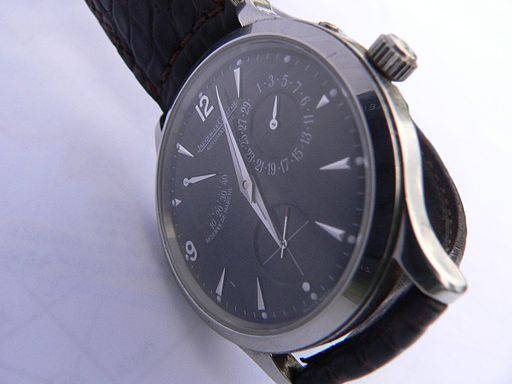
\includegraphics[width=0.75\textwidth]{img/watch.jpg}
  \end{minipage}
  % \end{textblock*}
    
  \vspace{-0.75cm}

  \begin{minipage}{0.45\textwidth}
    \hfill  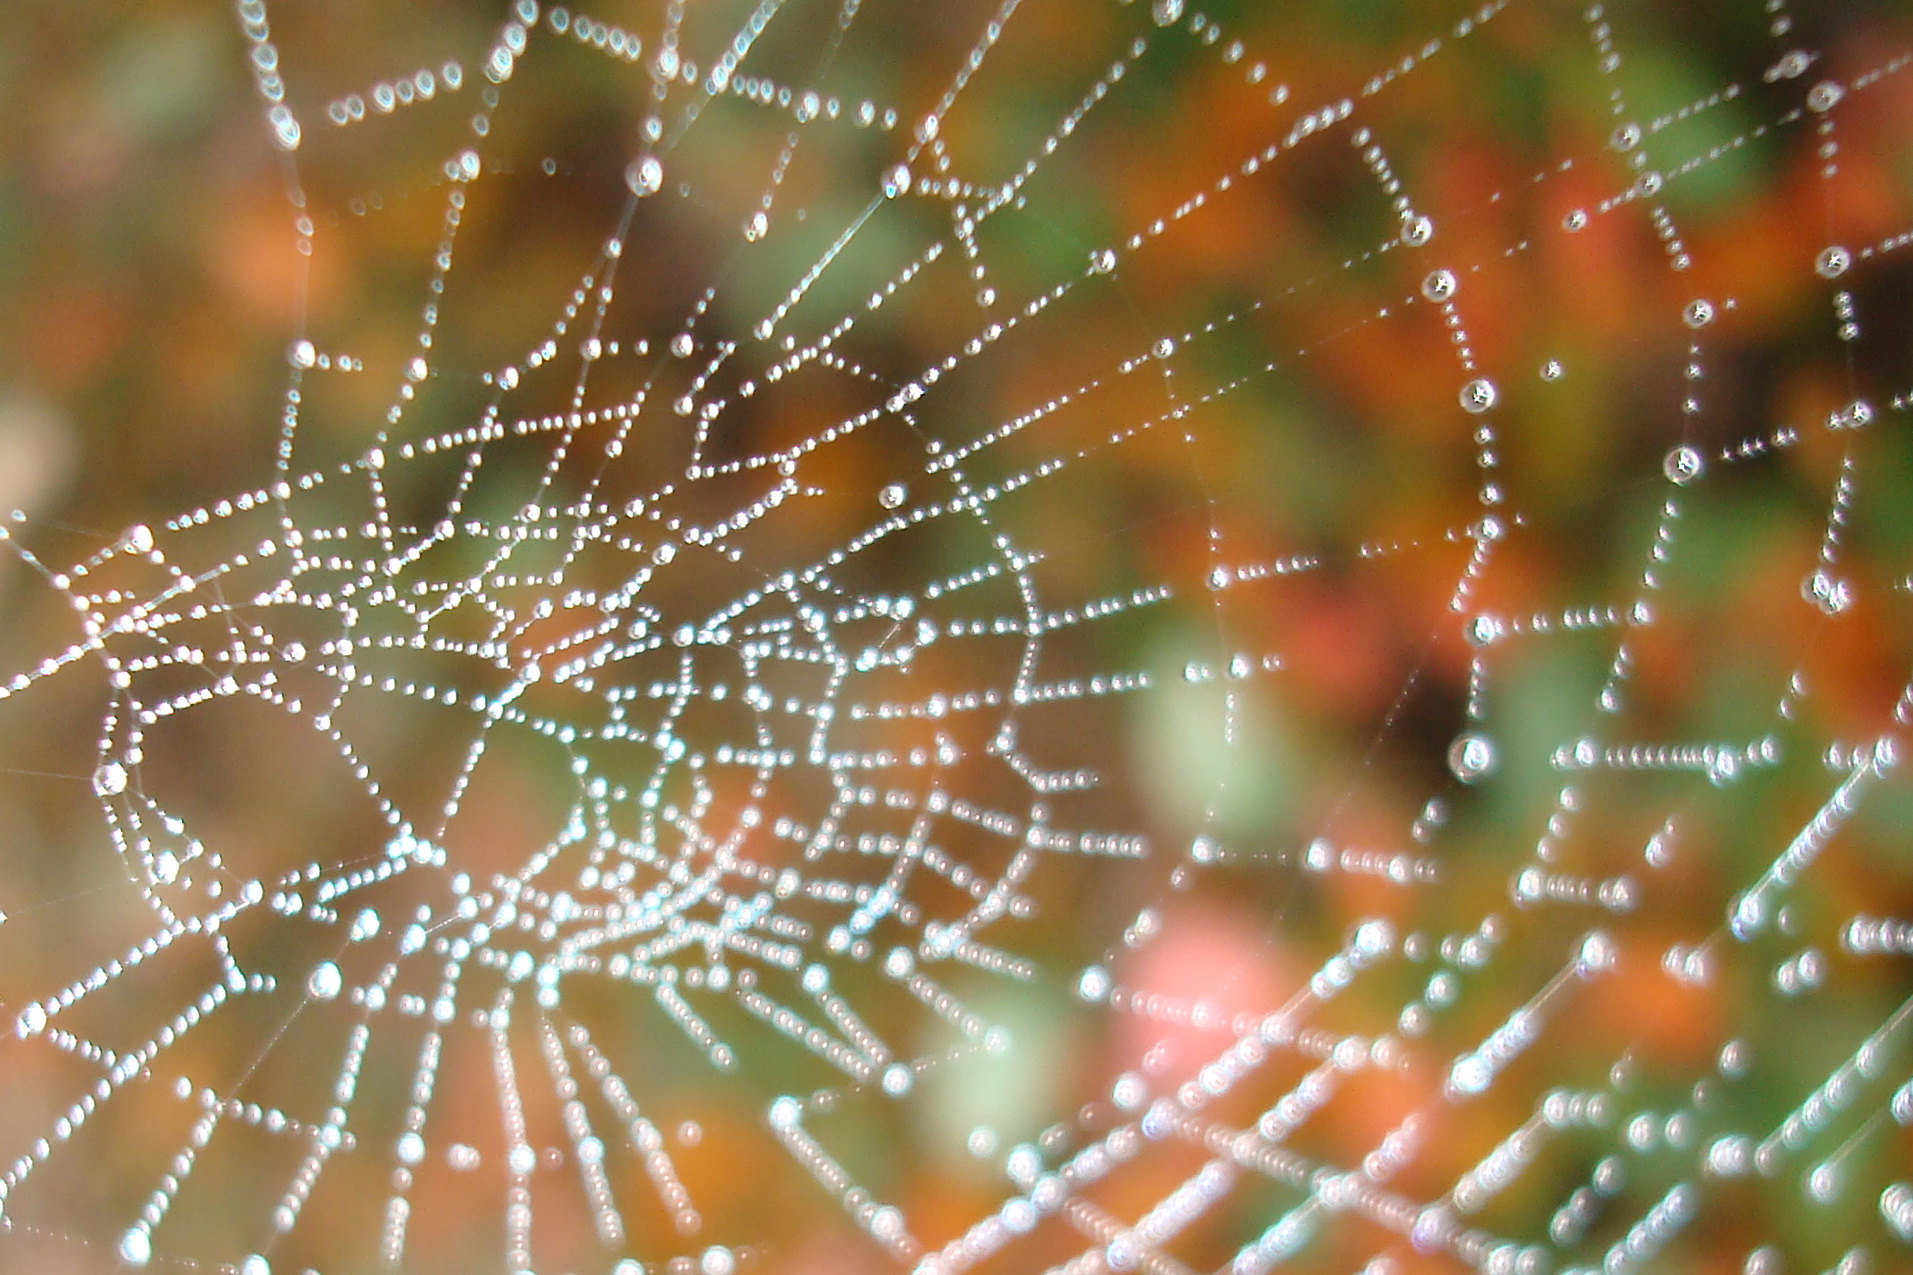
\includegraphics[width=0.8\textwidth]{img/toile.jpg}
  \end{minipage}  
  \begin{minipage}{0.45\textwidth}
    \textbf{Web} \YES{\cmark}
  \end{minipage}
  
  \vspace{-0.75cm}
  
  \begin{minipage}{0.45\textwidth}
    \hfill \NO{\xmark}\textbf{Sans fournisseur de services}
  \end{minipage}
  \begin{minipage}{0.45\textwidth}
    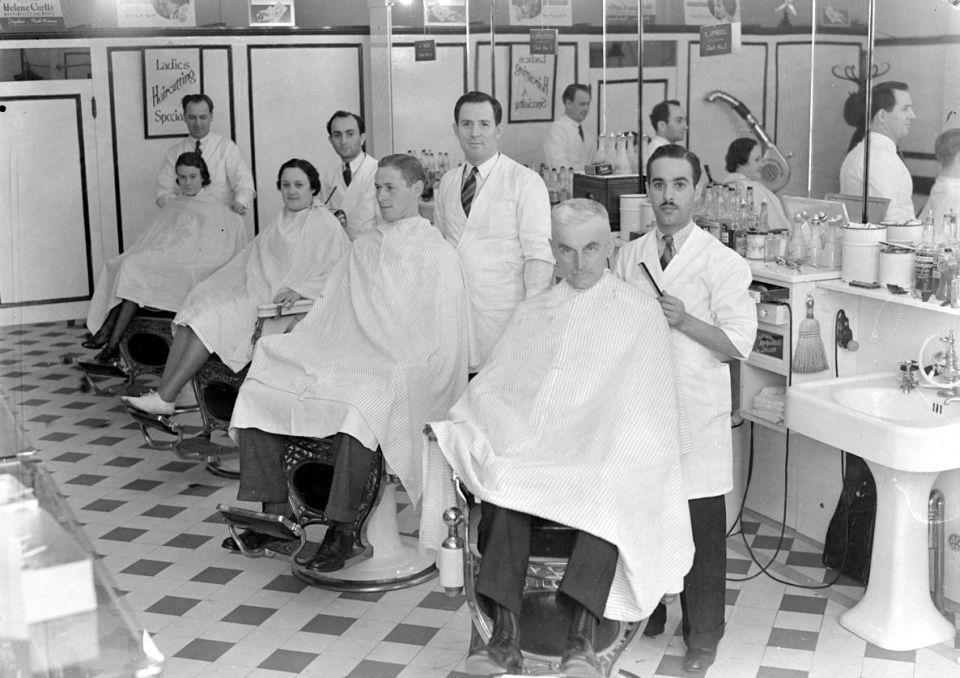
\includegraphics[width=0.8\textwidth]{img/service.jpg}
  \end{minipage}

  \vspace{-0.75cm}

  \begin{minipage}{0.45\textwidth}
    \hfill 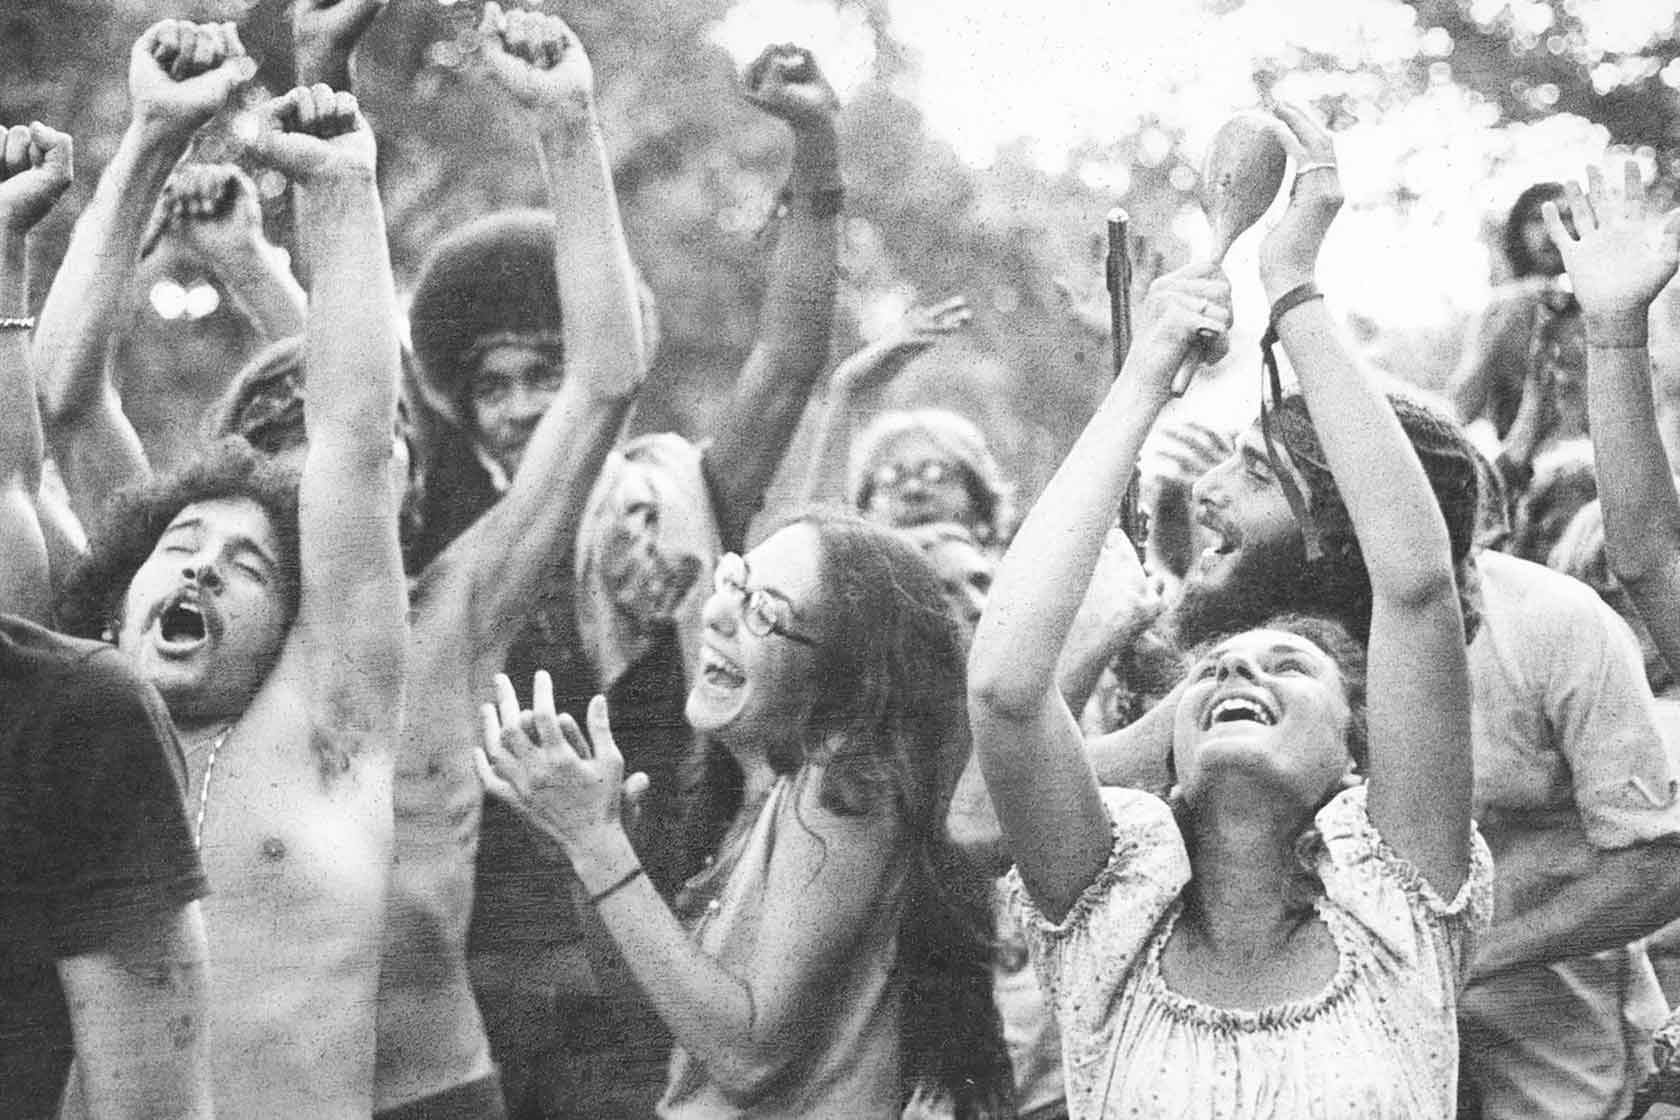
\includegraphics[width=0.8\textwidth]{img/crowd.jpg}
  \end{minipage}
  \begin{minipage}{0.45\textwidth}
    \textbf{Des milliers d'utilisateurs éditant simultanément} \NO{\xmark}
  \end{minipage}


%    \vspace{-4.5cm}\hspace{2cm}%
  \only<2>{
    \begin{tikzpicture}[remember picture,overlay]
      \draw (150pt,120pt) node
      [draw,align=left,fill=termithgreen!30,font=\large]{\textbf{L'édition
          collaborative temps réel}\\\textbf{est-elle possible sur le
          Web},\\\textbf{sans l'intervention d'un tiers}\\\textbf{et sans limites quant
        aux dimensions du système ?}};
    \end{tikzpicture}
  }
\end{frame}


\begin{frame}{Introduction}{Un éditeur collaboratif dans les navigateurs}
  

  \begin{minipage}{0.69\textwidth}
    \CRATE est un éditeur collaboratif 
    \begin{itemize}
    \item temps réel \YES{\cmark}
    \item fonctionnant dans les navigateurs Web \YES{\cmark}
    \item sans fournisseur de services \YES{\cmark}
    \item passant à l'échelle \YES{\cmark}
    \end{itemize}
  \end{minipage}
  \begin{minipage}{0.3\textwidth}
    
\includegraphics[width=\textwidth,interpolate=false]{img/crateicon.png}
  \end{minipage}
    
%  \vspace{1.0cm}
  
  \begin{textblock*}{1.18\textwidth}(-1cm,1cm)
    \animategraphics[loop,autoplay,width=1\textwidth]{10}{img/animations/tmp-}{0}{69}
  \end{textblock*}
  
  \vspace{1cm}

\end{frame}


\begin{frame}{Introduction}{Fonctionnement décentralisé}
  
  \hspace{-1cm}
  \begin{minipage}{0.42\textwidth}
    \begin{itemize}
      \item Chaque éditeur possède une copie locale du document;
      \vspace{0.5cm}
    \only<1>{\item Chaque caractère tapé est directement inséré dans la copie locale;}
    \only<2>{\item
      \textbf{Chaque caractère tapé est directement inséré dans la copie locale;}}
    \only<3->{\item Chaque caractère tapé est directement inséré dans la copie locale;}
    \only<1-2>{\item La modification est disséminée à l'ensemble du réseau;
    \item Les éditeurs recevant la modification l'appliquent.}
    \only<3->{\item \textbf{La modification est disséminée à l'ensemble du réseau;}
    \item \textbf{Les éditeurs recevant la modification l'appliquent;}}

    \end{itemize}
  \end{minipage}
  \begin{minipage}{0.56\textwidth}
    \begin{center}
      \begin{tikzpicture}

  \newcommand\X{50pt}
  \newcommand\Y{-20pt}
  
  \draw (0*\X, 0*\Y) node{
\includegraphics[width=16px]{img/crateicon.png}};
  \only<2->{\draw(0*\X, 0*\Y) node{\textbf{A}}};

  \draw (1*\X, -3*\Y) node{
\includegraphics[width=16px]{img/crateicon.png}};
  \draw (1*\X,  0*\Y) node{
\includegraphics[width=16px]{img/crateicon.png}};
  \draw (1*\X,  3*\Y) node{
\includegraphics[width=16px]{img/crateicon.png}};
  \only<3->{
  \draw (1*\X, -3*\Y) node{\textbf{A}};
  \draw (1*\X,  0*\Y) node{\textbf{A}};
  \draw (1*\X,  3*\Y) node{\textbf{A}};
  };

  \draw (2*\X, -4*\Y) node{
\includegraphics[width=16px]{img/crateicon.png}};
  \draw (2*\X, -3*\Y) node{
\includegraphics[width=16px]{img/crateicon.png}};
  \draw (2*\X, -2*\Y) node{
\includegraphics[width=16px]{img/crateicon.png}};

  \draw (2*\X, -1*\Y) node{
\includegraphics[width=16px]{img/crateicon.png}};
  \draw (2*\X,  0*\Y) node{
\includegraphics[width=16px]{img/crateicon.png}};
  \draw (2*\X,  1*\Y) node{
\includegraphics[width=16px]{img/crateicon.png}};

  \draw (2*\X,  2*\Y) node{
\includegraphics[width=16px]{img/crateicon.png}};
  \draw (2*\X,  3*\Y) node{
\includegraphics[width=16px]{img/crateicon.png}};
  \draw (2*\X,  4*\Y) node{
\includegraphics[width=16px]{img/crateicon.png}};

  \only<4->{
  \draw (2*\X, -4*\Y) node{\textbf{A}};
  \draw (2*\X, -3*\Y) node{\textbf{A}};
  \draw (2*\X, -2*\Y) node{\textbf{A}};

  \draw (2*\X, -1*\Y) node{\textbf{A}};
  \draw (2*\X,  0*\Y) node{\textbf{A}};
  \draw (2*\X,  1*\Y) node{\textbf{A}};

  \draw (2*\X,  2*\Y) node{\textbf{A}};
  \draw (2*\X,  3*\Y) node{\textbf{A}};
  \draw (2*\X,  4*\Y) node{\textbf{A}};
  };


  \draw[->] (6+0*\X, 0*\Y) -- (-6+1*\X, -3*\Y);
  \draw[->] (6+0*\X, 0*\Y) -- (-6+1*\X, 0*\Y);
  \draw[->] (6+0*\X, 0*\Y) -- (-6+1*\X,  3*\Y);

  \only<3>{\draw[->,very thick] (6+0*\X, 0*\Y) -- (-6+1*\X, -3*\Y);
    \draw[->, very thick] (6+0*\X, 0*\Y) -- (-6+1*\X, 0*\Y);
    \draw[->, very thick] (6+0*\X, 0*\Y) -- (-6+1*\X,  3*\Y);
  };


  \draw[->] (6+1*\X, -3*\Y) -- (-6+2*\X, -4*\Y);
  \draw[->] (6+1*\X, -3*\Y) -- (-6+2*\X, -3*\Y);
  \draw[->] (6+1*\X, -3*\Y) -- (-6+2*\X, -2*\Y);

  \draw[->] (6+1*\X, 0*\Y) -- (-6+2*\X, -1*\Y);
  \draw[->] (6+1*\X, 0*\Y) -- (-6+2*\X,  0*\Y);
  \draw[->] (6+1*\X, 0*\Y) -- (-6+2*\X,  1*\Y);

  \draw[->] (6+1*\X, 3*\Y) -- (-6+2*\X, 4*\Y);
  \draw[->] (6+1*\X, 3*\Y) -- (-6+2*\X, 3*\Y);
  \draw[->] (6+1*\X, 3*\Y) -- (-6+2*\X, 2*\Y);

  \only<4>{
  \draw[->,very thick] (6+1*\X, -3*\Y) -- (-6+2*\X, -4*\Y);
  \draw[->,very thick] (6+1*\X, -3*\Y) -- (-6+2*\X, -3*\Y);
  \draw[->,very thick] (6+1*\X, -3*\Y) -- (-6+2*\X, -2*\Y);

  \draw[->,very thick] (6+1*\X, 0*\Y) -- (-6+2*\X, -1*\Y);
  \draw[->,very thick] (6+1*\X, 0*\Y) -- (-6+2*\X,  0*\Y);
  \draw[->,very thick] (6+1*\X, 0*\Y) -- (-6+2*\X,  1*\Y);

  \draw[->,very thick] (6+1*\X, 3*\Y) -- (-6+2*\X, 4*\Y);
  \draw[->,very thick] (6+1*\X, 3*\Y) -- (-6+2*\X, 3*\Y);
  \draw[->,very thick] (6+1*\X, 3*\Y) -- (-6+2*\X, 2*\Y);
  };


  \draw (3*\X, 0*\Y) node{\ldots};

  \foreach \y in {0,...,36}
  {\draw(4*\X, {(-4.5+\y*0.25)*\Y})
    node{
\includegraphics[width=16px]{img/crateicon.png}};
    \only<5->{
      \draw(4*\X, {(-4.5+\y*0.25)*\Y}) node{\textbf{A}};
    }
  }
  % \draw (4*\X,  -4.5*\Y) node{
\includegraphics[width=16px]{img/crateicon.png}};
  % \draw (4*\X,  -4.25*\Y) node{
\includegraphics[width=16px]{img/crateicon.png}};
  % \draw (4*\X,  -4*\Y) node{
\includegraphics[width=16px]{img/crateicon.png}};
  % \draw (4*\X,  -3.75*\Y) node{
\includegraphics[width=16px]{img/crateicon.png}};
  % \draw (4*\X,  -3.5*\Y) node{
\includegraphics[width=16px]{img/crateicon.png}};
  % \draw (4*\X,  -3.25*\Y) node{
\includegraphics[width=16px]{img/crateicon.png}};


\end{tikzpicture}
    \end{center}
  \end{minipage}
  
  \vspace{0.4cm}
  \large
  \begin{itemize}
  \item [$\Rightarrow$] \textbf{taille de messages} $\times$ \textbf{nombre de messages}
  \end{itemize}

\end{frame}

\begin{frame}{Introduction}{Contributions}
  
  
  \begin{itemize}
  \item \textbf{taille des messages :} \LSEQ qui, dans le contexte de l'édition
    collaborative, borne la taille des messages de manière sous-linéaire par
    rapport au nombre d'insertions effectuées dans le document.
    \vspace{1cm}
  \item \textbf{nombre de messages :} \SPRAY qui s'adapte automatiquement à la
    taille du réseau de manière logarithmique et qui supporte le processus
    complexe d'établissement de connexion disponible dans les navigateurs Web.
  \end{itemize}

\end{frame}


% \begin{frame}{Introduction}{Éditeur collaboratif décentralisé}
  
%   \begin{center}
%     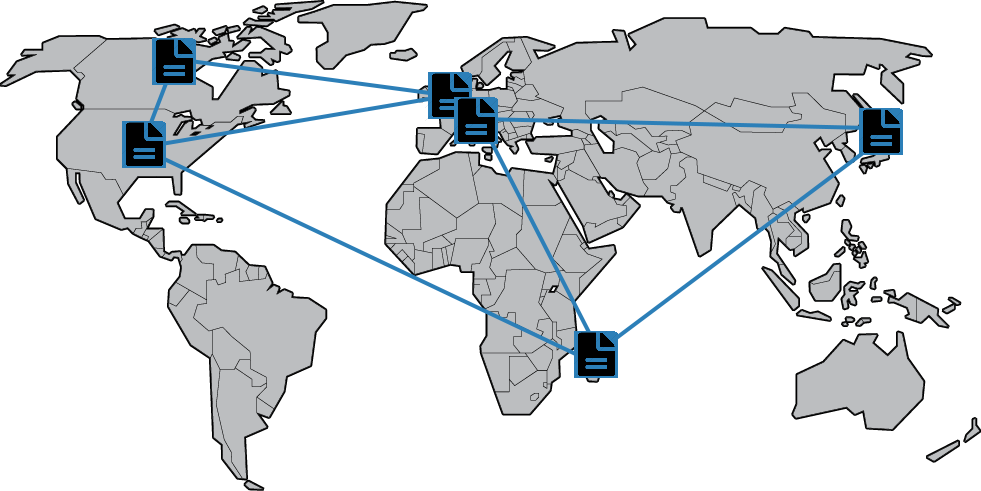
\includegraphics[width=0.8\textwidth]{img/world.png}
%   \end{center}

%   \vspace{0.25cm}

%   \begin{itemize}
%   \item [$\rightarrow$] Un éditeur collaboratif doit fonctionner sur les outils
%     informatiques les plus modestes (CPU, mémoire, \textbf{largeur de bande}).
%     \begin{itemize}
%     \item [$\rightarrow$] (taille des messages $\times$ nombre de messages)
%     \end{itemize}
%   \end{itemize}

%   \vspace{0.25cm}
  
%   \begin{enumerate}
%   \item Moyen de représenter efficacement un \textbf{document} de manière
%     \textbf{cohérente}; %\small{$\rightarrow$ taille des messages}
%   \item Moyen de \textbf{communiquer} efficacement les modifications sur le
%     document. %\small{$\rightarrow$ nombre de messages}
%   \end{enumerate}


%   % \begin{itemize}
%   % \item Répartition géographique des collaborateurs;
%   % \item Édition en temps réel.
%   % \end{itemize}
% \end{frame}


%%% Local Variables:
%%% mode: latex
%%% TeX-master: "../slides"
%%% End:


  \begin{frame}{Plan}
    \tableofcontents
  \end{frame}


  \section{Structure de séquences répartie à large échelle}

\begin{frame}{Structure de séquences}{Réplication}
  \vspace{-1.5cm}
  La \textbf{réplication optimiste} \REF{} améliore la \textbf{disponibilité} d'un
  document et sa \textbf{réactivité} aux changements effectués.
  \vspace{0.75cm}

  Fonctionnement :
  \begin{enumerate}[(a)]
  \item Une modification produit un résultat;
  \item ce résultat est disséminé aux autres répliques;
  \item ces dernières exécutent -- ou intègrent -- le résultat reçu.
  \end{enumerate}

  \begin{textblock*}{\textwidth}(-0.65cm,0.4cm) 
    
\begin{tikzpicture}[scale=0.95]

  \newcommand\X{30pt};
  \newcommand\Y{30pt};
  
  \draw[->](0pt,   0pt)--(10*\X,   0pt);
  \draw[->](0pt, -1*\Y)--(10*\X, -1*\Y);
  \draw[->](0pt, -2*\Y)--(10*\X, -2*\Y);
  
  \draw[fill=black](0pt, 0pt) node[anchor=east]{éditeur 1 }circle(2pt);
  \draw[fill=black](0pt, -1*\Y) node[anchor=east]{éditeur 2 }circle(2pt);
  \draw[fill=black](0pt, -2*\Y) node[anchor=east]{éditeur 3 }circle(2pt);

  \draw(\X,2pt)--node[anchor=south]{[WERTY]}( \X,   -2pt);
  \draw(\X,2 -1*\Y)--node[anchor=south]{[WERTY]}(\X,-2 -1*\Y);
  \draw(\X,2 -2*\Y)--node[anchor=south]{[WERTY]}(\X,-2 -2*\Y);
  \footnotesize
  \draw(3* \X,2pt)--node[anchor=north]
  {(a) \textsc{insert}(Q, 0) \DARKBLUE{\textbf{produit} $resultat$}}(3 * \X,   -2pt);
%  \draw(3* \X,2 -2*\Y)--node[anchor=north]{\textsc{delete}(\DARKBLUE{\textbf{0}})}(3 * \X,-2 -2*\Y);
  \normalsize

  \draw(3* \X,2pt)--node[anchor=south]{[QWERTY]}(3 * \X,   -2pt);
%  \draw(2* \X,2 -1*\Y)--node[anchor=south]{[ ]}(2* \X,-2 -1*\Y)
%  \draw(3* \X,2 -2*\Y)--node[anchor=south]{[ERTY]}( 3 * \X,-2 -2*\Y);

  \footnotesize
  \draw[->, dashed] (5*\X, 0pt) -- (15+7*\X, -1*\Y);
  \draw[->, dashed] (5*\X, 0pt)
  node[anchor = south west]{(b) \DARKBLUE{\textbf{dissémine}} $resultat$} -- (7*\X, -2*\Y);


  \draw (15+ 7*\X, 2-1*\Y) -- (15+ 7*\X, -2-1*\Y)
  node [anchor=north]{(c)};
  \draw (7*\X, 2-2*\Y) -- (7*\X, -2-2*\Y)
  node [anchor=north]{(c) \DARKBLUE{\textbf{intègre}} $resultat$ };
  \normalsize

%  \draw[->, dashed] (5*\X, -2*\Y) -- (7*\X,  0*\Y)
%  node[anchor=south]{\textsc{delete}(\DARKBLUE{\textbf{0}})};
%  \normalsize
%  \draw[->, dashed] (5*\X, -2*\Y) -- (7*\X, -1*\Y);

  \draw(9*\X, 2 -0*\Y)--node[anchor=south]{[QWERTY]}(9*\X,-2 -0*\Y);
  \draw(9*\X, 2 -1*\Y)--node[anchor=south]{[QWERTY]}(9*\X,-2 -1*\Y);
  \draw(9*\X, 2 -2*\Y)--node[anchor=south]{[QWERTY]}(9*\X,-2 -2*\Y);


%%  \draw(9*\X, 2 -0*\Y)--node[anchor=south]{[QWERTY]}(9*\X,-2 -0*\Y);
%%  \draw(9*\X, 2 -1*\Y)--node[anchor=south]{[QWERTY]}(9*\X,-2 -1*\Y);
%%  \draw(9*\X, 2 -2*\Y)--node[anchor=south]{[QWERTY]}(9*\X,-2 -2*\Y);


%%  \draw[fill=white, very thick]
%%  (0*\X, 0*\Y) node{$p_1$} +(-5pt,-5pt) rectangle +(5pt,5pt);
%%  \draw[->](-5+\X, 5+2*\Y)to[out=120,in=30](0pt,5+2*\Y); %% 6 -> 7
\end{tikzpicture}
  \end{textblock*}
\end{frame}


\begin{frame}{Structure de séquences}{Cohérence des répliques}
  
  \vspace{-1.5cm}

  D'après Sun et al. \REF{}, l'édition collaborative temps réel nécessite un
  système préservant les trois propriétés : 

  \begin{itemize}
  \item Convergence;
  \item Causalité;
  \item Intention.  
  \end{itemize}

  \begin{textblock*}{\textwidth}(-0.65cm,0.4cm) 
    
\begin{tikzpicture}[scale=0.95]

  \newcommand\X{30pt};
  \newcommand\Y{30pt};
  
  \draw[->](0pt,   0pt)--(10*\X,   0pt);
  \draw[->](0pt, -1*\Y)--(10*\X, -1*\Y);
  \draw[->](0pt, -2*\Y)--(10*\X, -2*\Y);
  
  \draw[fill=black](0pt, 0pt) node[anchor=east]{réplique 1 }circle(2pt);
  \draw[fill=black](0pt, -1*\Y) node[anchor=east]{réplique 2 }circle(2pt);
  \draw[fill=black](0pt, -2*\Y) node[anchor=east]{réplique 3 }circle(2pt);

  \draw(\X,2pt)--node[anchor=south]{[WERTY]}( \X,   -2pt);
  \draw(\X,2 -1*\Y)--node[anchor=south]{[WERTY]}(\X,-2 -1*\Y);
  \draw(\X,2 -2*\Y)--node[anchor=south]{[WERTY]}(\X,-2 -2*\Y);
  \footnotesize
  \draw(3* \X,2pt)--node[anchor=north]
  {\textsc{insert}(Q, 0)}(3 * \X,   -2pt);
%  \draw(3* \X,2 -2*\Y)--node[anchor=north]{\textsc{delete}(\DARKBLUE{\textbf{0}})}(3 * \X,-2 -2*\Y);
  \normalsize

  \draw(3* \X,2pt)--node[anchor=south]{[QWERTY]}(3 * \X,   -2pt);
%  \draw(2* \X,2 -1*\Y)--node[anchor=south]{[ ]}(2* \X,-2 -1*\Y)
%  \draw(3* \X,2 -2*\Y)--node[anchor=south]{[ERTY]}( 3 * \X,-2 -2*\Y);

  \footnotesize
  \draw[->, dashed] (4*\X, 0pt) -- (4.5*\X, -1*\Y);
  \draw[->, dashed] (4*\X, 0pt) to[out=25,in=155] (7.5*\X, 0pt)
  to[out=-40,in=95] (8.2*\X, -2*\Y);
  
  \draw(5.5*\X, 2-1*\Y)node[anchor=south]{\normalsize[WERTY]}--(5.5*\X, -2-1*\Y)
  node[anchor=north]{\footnotesize\textsc{delete}(0)};

  \draw[->, dashed] (6.5*\X, -1*\Y) -- (7*\X, -0*\Y);
  \draw[->, dashed] (6.5*\X, -1*\Y) -- (7*\X, -2*\Y);

  \draw[->, dashed, color=darkblue] (7*\X, -2*\Y) to[out=-45,in=-135]
  node[anchor=north]{\DARKBLUE{\textbf{attend}}} (8.5*\X, -2*\Y);

  \normalsize

%  \draw[->, dashed] (5*\X, -2*\Y) -- (7*\X,  0*\Y)
%  node[anchor=south]{\textsc{delete}(\DARKBLUE{\textbf{0}})};
%  \normalsize
%  \draw[->, dashed] (5*\X, -2*\Y) -- (7*\X, -1*\Y);

  \draw(9*\X, 2 -0*\Y)--node[anchor=south]{[WERTY]}(9*\X,-2 -0*\Y);
  \draw(9*\X, 2 -1*\Y)--node[anchor=south]{[WERTY]}(9*\X,-2 -1*\Y);
  \draw(9*\X, 2 -2*\Y)--node[anchor=south]{[WERTY]}(9*\X,-2 -2*\Y);


%%  \draw(9*\X, 2 -0*\Y)--node[anchor=south]{[QWERTY]}(9*\X,-2 -0*\Y);
%%  \draw(9*\X, 2 -1*\Y)--node[anchor=south]{[QWERTY]}(9*\X,-2 -1*\Y);
%%  \draw(9*\X, 2 -2*\Y)--node[anchor=south]{[QWERTY]}(9*\X,-2 -2*\Y);


%%  \draw[fill=white, very thick]
%%  (0*\X, 0*\Y) node{$p_1$} +(-5pt,-5pt) rectangle +(5pt,5pt);
%%  \draw[->](-5+\X, 5+2*\Y)to[out=120,in=30](0pt,5+2*\Y); %% 6 -> 7
\end{tikzpicture}
  \end{textblock*}

\end{frame}


\begin{frame}{Structure de séquences}{Intention}
  
  L'effet observé sur le document lors de la génération d'une opération doit
  être également observé lors de son intégration malgré l'interférence
  d'opérations \textbf{concurrentes}.

  \vspace{0.5cm}

  \begin{itemize}
  \item Difficile à formaliser dans le cas général;
  \item L'opération doit respecter le plus possible sa spécification séquentielle \REF.
  \end{itemize}

  \vspace{0.5cm}
  
  Pour la séquence :
  \begin{itemize}
  \item \og insérer l'élément $e$ à la position $i$ dans la séquence \fg
  \item \og supprimer l'élément à la position $i$ dans la séquence \fg
  \end{itemize}

  \vspace{0.5cm}

  \begin{itemize}
    \only<1-1>{\item [$\rightarrow$]L'intention semble être liée à aux
      positions.}
    \only<2->{\item [$\rightarrow$]\sout{L'intention semble être
        liée aux \textbf{positions}.}}
    \uncover<2->{\item [$\rightarrow$] Une séquence
    se définit par un \textbf{ordre dense} sur ses éléments : les éléments 
    sont ordonnés
    et il est toujours possible d'insérer un élément entre deux autres éléments.}
  \end{itemize}
  
\end{frame}

\begin{frame}{Structure de séquences}{Spécification}
  \begin{definition}[Spécification séquentielle d'une séquence]
  Soit une série d'opérations $H$ produisant la séquence
  $s(H) = \{p_1,\, p_2 \ldots p_k\}$ avec $p_{1..k} \in \mathcal{P}$ où
  $\mathcal{P}$ est un ensemble muni d'un ordre
  dense $(\mathcal{P},\,<_\mathcal{P})$ tel que : \\
  $\forall p\in\mathcal{P},\, p_\vdash <_\mathcal{P} p <_\mathcal{P} p_\dashv $
  \hfill et \ \
  $p_\vdash <_\mathcal{P} p_1 <_\mathcal{P} p_2 <_\mathcal{P} \ldots
  <_\mathcal{P} p_k <_\mathcal{P} p_\dashv$.
  
  \vspace{0.25cm}

  \noindent L'insertion d'un élément $e$ en position $i$ dans la séquence $s(H)$
  est définie de la façon suivante :
  \begin{equation}
    \small
    s(H \cup INSERT(i,\, e)) \rightarrow s(H) \cup 
    \begin{cases}
      \{p,\, p_\vdash <_\mathcal{P} p <_\mathcal{P} p_\dashv \} & i = 0 \wedge |s(H)| = 0\\
      \{p,\, p_\vdash <_\mathcal{P} p <_\mathcal{P} p_1 \} & i = 0 \wedge |s(H)|>0\\
      \{p,\, p_k <_\mathcal{P} p <_\mathcal{P} p_\dashv \} & i = k\\
      \{p,\, p_i <_\mathcal{P} p <_\mathcal{P} p_{i+1} \} & sinon
    \end{cases}
  \end{equation}

  \noindent La suppression de l'élément en position $i$ dans la séquence $s(H)$
  est définie de la façon suivante :
  \begin{equation}
    \small
    s(H \cup DELETE(i)) \rightarrow s(H) \setminus \{ p_i \}
  \end{equation}
\end{definition}
\end{frame}


\begin{frame}{Structure de séquences}{Complexités}

\begin{itemize}
  \only<1-1>{\item Complexité en \textbf{communication};}
  \only<2->{\item  \textbf{Complexité en communication};}
\item Complexité \textbf{spatiale} de la réplique;
\item Complexité \textbf{temporelle} d'une opération \textbf{générée} localement;
  \only<1-1>{\item Complexité \textbf{temporelle} de l'\textbf{intégration} d'une opération reçue.}
  \only<2->{\item \textbf{Complexité temporelle de l'intégration d'une opération reçue.}}
\end{itemize}

%% (TODO) maybe explain the reasons of this emphasis
\end{frame}


% \begin{frame}{Structure de séquences}{État de l'art : transformées opérationnelles}

%   \vspace{-1.5cm}

%   Ces approches \REF{} ont une signature identique à celle communément employée
%   pour les séquences : 
%   \begin{itemize}
%   \item \textsc{insert}($element,\,position$)
%   \item \textsc{delete}($position$)
%   \end{itemize}

%   \vspace{0.5cm}

%   Lors de la réception d'une opération, ses arguments sont ajustés afin qu'ils
%   s'appliquent à l'état courant de la réplique malgré les opérations effectuées
%   et intégrées en concurrence. 


%   \begin{textblock*}{\textwidth}(-0.65cm,0.4cm) 
%     
\begin{tikzpicture}[scale=0.95]

  \newcommand\X{30pt};
  \newcommand\Y{30pt};
  
  \draw[->](0pt,   0pt)--(10*\X,   0pt);
  \draw[->](0pt, -1*\Y)--(10*\X, -1*\Y);
  \draw[->](0pt, -2*\Y)--(10*\X, -2*\Y);
  
  \draw[fill=black](0pt, 0pt) node[anchor=east]{réplique 1 }circle(2pt);
  \draw[fill=black](0pt, -1*\Y) node[anchor=east]{réplique 2 }circle(2pt);
  \draw[fill=black](0pt, -2*\Y) node[anchor=east]{réplique 3 }circle(2pt);

  \draw(\X,2pt)--node[anchor=south]{[WERTY]}( \X,   -2pt);
  \draw(\X,2 -1*\Y)--node[anchor=south]{[WERTY]}(\X,-2 -1*\Y);
  \draw(\X,2 -2*\Y)--node[anchor=south]{[WERTY]}(\X,-2 -2*\Y);
  \footnotesize
  \draw(3* \X,2pt)--node[anchor=north]{\textsc{insert}(Q, 0)}(3 * \X,   -2pt);
  \draw(3* \X,2 -2*\Y)--node[anchor=north]{\textsc{delete}(\DARKBLUE{\textbf{0}})}(3 * \X,-2 -2*\Y);
  \normalsize

  \draw(3* \X,2pt)--node[anchor=south]{[QWERTY]}(3 * \X,   -2pt);
%  \draw(2* \X,2 -1*\Y)--node[anchor=south]{[ ]}(2* \X,-2 -1*\Y)
  \draw(3* \X,2 -2*\Y)--node[anchor=south]{[ERTY]}( 3 * \X,-2 -2*\Y);

  \draw[->, dashed] (5*\X, 0pt) -- (7*\X, -1*\Y);
  \draw[->, dashed] (5*\X, 0pt) -- (7*\X, -2*\Y);

  \footnotesize
  \draw[->, dashed] (5*\X, -2*\Y) -- (7*\X,  0*\Y)
  node[anchor=south]{\textsc{delete}(\DARKBLUE{\textbf{1}})};
  \normalsize
  \draw[->, dashed] (5*\X, -2*\Y) -- (7*\X, -1*\Y);

  \draw(9*\X, 2 -0*\Y)--node[anchor=south]{[QERTY]}(9*\X,-2 -0*\Y);
  \draw(9*\X, 2 -1*\Y)--node[anchor=south]{[QERTY]}(9*\X,-2 -1*\Y);
  \draw(9*\X, 2 -2*\Y)--node[anchor=south]{[QERTY]}(9*\X,-2 -2*\Y);


%%  \draw(9*\X, 2 -0*\Y)--node[anchor=south]{[QWERTY]}(9*\X,-2 -0*\Y);
%%  \draw(9*\X, 2 -1*\Y)--node[anchor=south]{[QWERTY]}(9*\X,-2 -1*\Y);
%%  \draw(9*\X, 2 -2*\Y)--node[anchor=south]{[QWERTY]}(9*\X,-2 -2*\Y);


%%  \draw[fill=white, very thick]
%%  (0*\X, 0*\Y) node{$p_1$} +(-5pt,-5pt) rectangle +(5pt,5pt);
%%  \draw[->](-5+\X, 5+2*\Y)to[out=120,in=30](0pt,5+2*\Y); %% 6 -> 7
\end{tikzpicture}
%   \end{textblock*}
% \end{frame}


\begin{frame}{Structure de séquences}{Le prix de la causalité}
  
  Ordonner les opérations selon l'ordre causal est extrêmement coûteux : au
  minimum $\mathcal{O}(W)$ en communication où $W$ est le nombre de participants
  ayant jamais écrit dans le document \REF.
  \begin{itemize}
  \item[$\rightarrow$] Relaxer l'ordre est nécessaire pour le passage à l'échelle
  \end{itemize}
  
  \vspace{0.5cm}
  
  \large
  \begin{itemize}
  \item [$\rightarrow$] L'utilisation de structures de données répliquées sans
    conflits \REF permet cela.
    \begin{itemize}
    \item [$\rightarrow$] Ces approches se basent sur la génération
      d'identifiants uniques et immuables. Nous nous intéresserons
      particulièrement à celles dont les identifiants sont des listes de taille
      variable.
    \end{itemize}
  \end{itemize}

\end{frame}

\begin{frame}{Structure de séquences}{Structures sans conflits}
  
  La signature change : 
  \begin{itemize}
  \item \textsc{insert}($element,\, position$) $\rightarrow$
    \textsc{insert}($id_{position-1},\, element,\, id_{position}$)
  \item \textsc{delete}($position$) $\rightarrow$ \textsc{delete}($id_{position}$)
  \end{itemize}

  \vspace{0.5cm}
  

  \begin{algorithm}[H]
    
\footnotesize
\algrenewcommand{\algorithmiccomment}[1]{\hskip2em$\rhd$ #1}

\newcommand{\comment}[1]{$\rhd$ #1}


\algblockdefx[initially]{initially}{endInitially}
  [0] {\textbf{INITIALLY:}} 

\algblockdefx[local]{local}{endLocal}
  [0] {\textbf{LOCAL UPDATE:}}

\algsetblockdefx[received]{received}{endReceived}
  {65535}{}
  [0] {\textbf{RECEIVED UPDATE:}}

\algblockdefx[onInsert]{onLocal}{endOnLocal}
  [0] {\textbf{on} insert ($previous \in \mathcal{I},\,\alpha \in \mathcal{A},\,
   next\in\mathcal{I}$):}
  [0] {\textbf{on} delete ($i \in \mathcal{I}$):} 

\algsetblockdefx[onRemote]{onRemote}{endOnRemote}
  {65535}{}
  [0] {\textbf{on} insert ($i\in\mathcal{I}$):
    \hfill\comment{\DARKBLUE{\textbf{une fois}} par identifiant}}
  [0] {\textbf{on} delete ($i\in\mathcal{I}$):
    \hfill\comment{\DARKBLUE{\textbf{après}} l'exécution de \textsc{insert}($i$)}} 

\newcommand{\LINEFOR}[2]{%
  \algorithmicfor\ {#1}\ \algorithmicdo\ {#2} %
  }

\newcommand{\LINEIFTHEN}[2]{%
  \algorithmicif\ {#1}\ \algorithmicthen\ {#2} %
  }

\newcommand{\INDSTATE}[1][1]{\State\hspace{\algorithmicindent}}

\begin{algorithmic}[1]
  \Statex
  \initially
    \State $T \leftarrow \varnothing$;
    \hfill \comment{CRDT conçue pour les séquences}
  \endInitially
  
  \local
    \onLocal
    \State \textbf{let}
    $\langle p,\, q \rangle \leftarrow $\textsc{convert2Path}$(previous,\, next)$;
    \State \textbf{let}
    $\DARKBLUE{newPath \leftarrow} $\DARKBLUE{\textbf{\textsc{allocPath}}}\DARKBLUE{$(p,\,q)$}; \label{line:allocpath}
    \State \textbf{let} 
    $newDis \leftarrow $\textsc{allocDis}$(p,\, newPath,\, q)$; \label{line:allocdes}
    \State \textsc{broadcast}$(\text{'insert'},\,
    \langle newPath,\, \alpha,\, newDis \rangle)$;
    \endOnLocal
    \INDSTATE \textsc{broadcast}$(\text{'delete'},\,i)$;
  \endLocal
  
  \received
    \onRemote
    \State $T \leftarrow T \cup i$;
    \endOnRemote
    \INDSTATE $T \leftarrow T\, \backslash\, i$; 
  
\end{algorithmic}

  \end{algorithm}

\end{frame}


\begin{frame}{Structure de séquences}{Problèmes d'allocation}

  La fonction d'allocation ne connait ni le \textbf{nombre} de caractères, ni
  leur \textbf{position} dans la séquence finale.

  \vspace{0.5cm}

  \begin{center}
    \begin{tikzpicture}

  \draw(-4,1)node{0};

  \draw[hide on=1-5, bold on=6](-3,1)node{0.0.0.1};
  \draw[hide on=1-4, bold on=5](-2,1)node{0.0.1};
  \draw[hide on=1-3, bold on=4](-1,1)node{0.1};
  \draw[bold on=1](0,1)node{1};
  \draw[hide on=1, bold on=2](1,1)node{2};
  \draw[hide on=1-2,bold on=3](2,1)node{3};
%  \draw[hide on=1-2,bold on=3](3,1)node{8};
%  \draw[hide on=1-3,bold on=4](4,1)node{8.1};

  \draw(5,1)node{9};

  \draw[hide on=1-5, bold on=6](-3,0)node{Q};
  \draw[hide on=1-4, bold on=5](-2,0)node{W};
  \draw[hide on=1-3, bold on=4](-1,0)node{E};
  \draw[bold on=1](0,0)node{R};
  \draw[hide on=1, bold on=2](1,0)node{T};
  \draw[hide on=1-2, bold on=3](2,0)node{Y};
%  \draw[hide on=1-2, bold on=3](3,0)node{E};
%  \draw[hide on=1-2, bold on=3](4,0)node{S};


\end{tikzpicture}
  \end{center}

\end{frame}


\begin{frame}{Structure de séquences}{Arbre}
  
  \begin{center}
    \begin{tikzpicture}[scale=1.2]

\newcommand\Y{-30}
\newcommand\ADDY{-8}


  %% node to node
  \small
  \draw[thick] (0pt,0pt) -- node[anchor=south east]{\DARKBLUE{0}} (-40pt,\Y pt);
  \draw[thick] (0pt,0pt) -- node[anchor=east]{3} (30pt, \Y pt); %% Y
  \draw[thick] (0pt, 0 pt) -- node[anchor=east]{2} (15pt, 1 * \Y pt); %% T
  \draw[thick] (-40pt, \Y pt) -- node[anchor=east]{\DARKBLUE{0}} (-40pt, 2 * \Y pt); %% 0
  \draw[thick] (0pt, 0 pt) -- node[anchor=east]{1} (0pt, 1 * \Y pt); %% R
  \draw[thick] (-40pt, 2*\Y pt)-- node[anchor=east]{\DARKBLUE{0}}(-40pt, 3 * \Y pt); %% 0
  \draw[thick] (-40pt, 1*\Y pt) -- node[anchor=north]{1}(-15pt, 2*\Y pt); %% E
  % \draw[thick] (-40pt, 3*\Y pt) -- node[anchor=east]{\DARKBLUE{0}}(-40pt,4 * \Y pt); %% 0
  \draw[thick] (-40pt, 2*\Y pt) -- node[anchor=north]{1}(-25pt, 3* \Y pt); %% W
  % \draw[thick] (-40pt, 4*\Y pt) -- node[anchor=east]{\DARKBLUE{0}}(-40pt,5 * \Y pt); %% 0
  \draw[thick] (-40pt, 3*\Y pt) -- node[anchor=east]{\DARKBLUE{1}}(-35pt, 4*\Y pt); %% Q

  \draw[dashed, thick] (0pt,0pt) -- node[anchor=south west]{9} (40pt,\Y pt);

  %% node to element
  \draw[->] ( 30pt, \Y pt) -- ( 30pt, \ADDY + \Y pt); %% Y
  \draw[->] ( 15pt, 1* \Y pt) -- ( 15pt, \ADDY +  1*\Y pt); %% T
  \draw[->] (  0pt, 1 *\Y pt) -- (  0pt, \ADDY +  1 *\Y pt); %% R
  \draw[->] (-15pt, 2 *\Y pt) -- ( -15pt, \ADDY + 2 *\Y pt); %% E
  \draw[->] (-25pt, 3 *\Y pt) -- ( -25pt, \ADDY + 3 *\Y pt); %% W
  \draw[->] (-35pt, 4 *\Y pt) -- ( -35pt, \ADDY + 4 *\Y pt); %% Q

  %% element to desambiguator
  % \draw[->,densely dashdotted]
  % ( 30pt, \ADDY + \Y pt) -- ( 30pt,2.75*\ADDY+\Y pt); %% Y
  % \draw[->,densely dashdotted]
  % ( 15pt, \ADDY + 2* \Y pt) -- ( 15pt,2.75*\ADDY+ 2* \Y pt); %% T
  % \draw[->,densely dashdotted]
  % ( 0pt, \ADDY + 3* \Y pt) -- (  0pt,2.75*\ADDY+ 3* \Y pt); %% R
  % \draw[->,densely dashdotted]
  % ( -15pt, \ADDY + 4 *\Y pt) -- ( -15pt,2.75*\ADDY+ 4* \Y pt); %% E
  % \draw[->,densely dashdotted]
  % ( -25pt, \ADDY + 5 *\Y pt) -- ( -25pt,2.75*\ADDY+ 5*\Y pt); %% W
  % \draw[->,densely dashdotted]
  % ( -35pt, \ADDY + 6* \Y pt) -- ( -35pt,2.75*\ADDY+ 6*\Y pt); %% Q

  %% node
 \draw[fill=black] (0pt,0pt) circle (1pt); %% rooot
  \draw[fill=white] ( 30pt, \Y pt) circle (1pt); %% Y
  \draw[fill=white] (-40pt, \Y pt) circle (1pt); %% 0
  \draw[fill=white] ( 15 pt, 1 * \Y pt) circle (1pt); %% T
  \draw[fill=white] (-40pt, 2 * \Y pt) circle (1pt); %% 0
  \draw[fill=white] (  0 pt, 1 * \Y pt) circle (1pt); %% R
  \draw[fill=white] (-40pt, 3 * \Y pt) circle (1pt); %% 0
  \draw[fill=white] (-15 pt, 2 * \Y pt) circle (1pt); %% E
%  \draw[fill=white] (-40pt, 4 * \Y pt) circle (1pt); %% 0
  \draw[fill=white] (-25 pt, 3 * \Y pt) circle (1pt); %% W
%  \draw[fill=white] (-40pt, 5 * \Y pt) circle (1pt); %% 0
  \draw[fill=white] (-35 pt, 4 * \Y pt) circle (1pt); %% Q

  \draw[fill=black] ( 40pt, \Y pt) circle (1pt);


  %% elements
  \draw[fill=white] ( 30pt, -4 + \ADDY + \Y pt)
  node{\textbf{Y}} +(-4pt,-4pt) rectangle +(4pt,4pt) ; %% Y
  \draw[fill=white] ( 15pt, -4 + \ADDY +  1 *\Y pt)
  node{\textbf{T}} +(-4pt,-4pt) rectangle +(4pt,4pt) ; %% T
  \draw[fill=white] (  0pt, -4 + \ADDY +  1* \Y pt)
  node{\textbf{R}} +(-4pt,-4pt) rectangle +(4pt,4pt) ; %% R
  \draw[fill=white] (-15pt, -4 + \ADDY + 2 *\Y pt)
  node{\textbf{E}} +(-4pt,-4pt) rectangle +(4pt,4pt) ; %% E
  \draw[fill=white] (-25pt, -4 + \ADDY + 3 * \Y pt)
  node{\textbf{W}} +(-4pt,-4pt) rectangle +(4pt,4pt) ; %% W
  \draw[fill=white] (-35pt, -4 + \ADDY + 4 *\Y pt)
  node{\textbf{Q}} +(-4pt,-4pt) rectangle +(4pt,4pt) ; %% Q

  %% desambiguator
  % \draw[fill=gray!20]( 30pt, -2.5 + 2.75 * \ADDY + \Y pt)
  % +(-2.5pt,-2.5pt) rectangle +(2.5pt,2.5pt);
  % \draw[fill=gray!20]( 15pt, -2.5 + 2.75 * \ADDY +2 *\Y pt)
  % +(-2.5pt,-2.5pt) rectangle +(2.5pt,2.5pt);
  % \draw[fill=gray!20](  0pt, -2.5 + 2.75 * \ADDY + 3*\Y pt)
  % +(-2.5pt,-2.5pt) rectangle +(2.5pt,2.5pt);
  % \draw[fill=gray!20](-15pt, -2.5 + 2.75 * \ADDY +4*\Y pt )
  % +(-2.5pt,-2.5pt) rectangle +(2.5pt,2.5pt);
  % \draw[fill=gray!20](-25pt, -2.5 + 2.75 * \ADDY + 5*\Y pt)
  % +(-2.5pt,-2.5pt) rectangle +(2.5pt,2.5pt);
  % \draw[fill=gray!20](-35pt, -2.5 + 2.75 * \ADDY +6*\Y pt) 
  % +(-2.5pt,-2.5pt) rectangle +(2.5pt,2.5pt);

  %% insertion order
  \draw[->,dashed, color=darkblue] (0pt, 1.75 * \Y pt) node[anchor=north west, align=left]{\ \ \DARKBLUE{ordre}\\ \DARKBLUE{d'insertion}} --  (45pt, 1.75 * \Y pt);

  \draw[->,dashed, color=darkblue] (0pt, 1.75 * \Y pt) -- (-25pt, 4.75 * \Y pt);

\end{tikzpicture}

  \end{center}
  
  \vspace{0.5cm}
  
  La taille des chemins impacte les performances de l'éditeur et le trafic
  généré par l'éditeur.
  \begin{itemize}
  \item [$\rightarrow$] \textsc{allocPath} doit allouer les plus petits chemins
    possibles.
  \end{itemize}

\end{frame}


\begin{frame}{Structure de séquences}{Définition du problème}

  \begin{problem}
    Soit la séquence d'identifiants $s(I)= id_1.id_2\ldots id_I$, et
    $s(I+1) = s(I) \cup $\textsc{insert}$(p,\, \_,\, n)$ où $p,q \in s(I)$ et
    $p<_\mathcal{I}q$. Soit $|s(I)|$ la taille de la représentation binaire de la
    séquence. La fonction \textsc{insert} doit allouer des identifiants tels que :
    \begin{equation}
      |s(I+1)| - |s(I)| < \mathcal{O}(I)
    \end{equation}
  \end{problem}
  
  \vspace{0.5cm}

  \begin{itemize}
  \item [$\rightarrow$] Sinon, il faut relocaliser les identifiants qui ont été
    générés pour conserver de bonnes performances
    \begin{itemize}
    \item [$\approx$] consensus répartis qui ne passe pas à l'échelle.
    \end{itemize}
  \end{itemize}

\end{frame}


\begin{frame}{Structure de séquences}{\LSEQ}
  
  Fonction d'allocation de chemins :
  \begin{enumerate}
  \item Une structure d'arbre dont l'arité maximale augmente avec la profondeur;
  \item Deux sous-fonctions d'allocation conçues pour gérer des comportements
    d'édition opposés;
  \item Une fonction assignant à chaque profondeur de l'arbre une sous-fonction
    d'allocation parmi celles disponibles.
  \end{enumerate}
  
\end{frame}


\begin{frame}{Structure de séquences}{Arbre exponentiel}

  \begin{center}
    
\begin{tikzpicture}[scale=1.3]

\newcommand\X{20pt}
\newcommand\Y{-20pt}

\newcommand\ADDYA{-10pt}
\newcommand\ADDYB{-30pt}

%\draw (-0.5*\X, 0*\Y); %% spacing

\draw[color=darkblue] (0*\X, 0*\Y) -- node[anchor=west]{1 bit}( 1*\X, 1*\Y);
\draw[dashed] (0*\X, 0*\Y) -- ( -1*\X, 1*\Y);

\draw[fill=black] (0*\X, 0*\Y) circle (1pt);
\draw[fill=white] (-1*\X, 1*\Y) circle (1pt); 

%% 
\draw[dashed] (1*\X, 1*\Y) -- (1.25*\X, \ADDYA + 2*\Y);
\draw[dashed] (1*\X, 1*\Y) -- (1.5*\X, \ADDYA + 2*\Y);
\draw[dashed] (1*\X, 1*\Y) -- (1.75*\X, \ADDYA + 2*\Y);
\draw[color=darkblue] (1*\X, 1*\Y) -- node[anchor=west]{2 bits} (2*\X, \ADDYA + 2*\Y);

\draw[fill=white] (1*\X, 1*\Y) circle (1pt); 
%%

\draw[dashed](2*\X, \ADDYA + 2*\Y) -- (2.125*\X, \ADDYB + 3*\Y);
\draw[dashed](2*\X, \ADDYA + 2*\Y) -- (2.25*\X, \ADDYB + 3*\Y);
\draw[dashed](2*\X, \ADDYA + 2*\Y) -- (2.375*\X, \ADDYB + 3*\Y);
\draw[dashed](2*\X, \ADDYA + 2*\Y) -- (2.5*\X, \ADDYB + 3*\Y);
\draw[dashed](2*\X, \ADDYA + 2*\Y) -- (2.625*\X, \ADDYB + 3*\Y);
\draw[dashed](2*\X, \ADDYA + 2*\Y) -- (2.75*\X, \ADDYB + 3*\Y);
\draw[dashed](2*\X, \ADDYA + 2*\Y) -- (2.875*\X, \ADDYB + 3*\Y);
\draw[color=darkblue](2*\X, \ADDYA + 2*\Y) -- node[anchor=west]{3 bits} (3*\X, \ADDYB + 3*\Y);


\draw[fill=white] (1.25*\X, \ADDYA + 2*\Y) circle (1pt);
\draw[fill=white] (1.5 *\X, \ADDYA + 2*\Y) circle (1pt);
\draw[fill=white] (1.75*\X, \ADDYA + 2*\Y) circle (1pt);
\draw[fill=white] (2*\X, \ADDYA + 2*\Y) circle (1pt);

%%

\draw[fill=white] (2.125*\X, \ADDYB + 3*\Y) circle (1pt);
\draw[fill=white] (2.25*\X, \ADDYB + 3*\Y) circle (1pt);
\draw[fill=white] (2.375*\X, \ADDYB + 3*\Y) circle (1pt);
\draw[fill=white] (2.5*\X, \ADDYB + 3*\Y) circle (1pt);
\draw[fill=white] (2.625*\X, \ADDYB + 3*\Y) circle (1pt);
\draw[fill=white] (2.75*\X, \ADDYB + 3*\Y) circle (1pt);
\draw[fill=white] (2.875*\X, \ADDYB + 3*\Y) circle (1pt);
\draw[fill=white] (3*\X, \ADDYB + 3*\Y) 
node[anchor=north west]{\DARKBLUE{[1.3.7]}} circle (1pt);



\end{tikzpicture}
  \end{center}

\end{frame}


\begin{frame}{Structure de séquences}{Sous-fonctions d'allocations}
  
  \begin{minipage}{0.45\textwidth}
    \begin{center}
      \begin{tikzpicture}[scale=1]

  %% node to node
  \scriptsize
  \draw[dashed, thick] (0pt,0pt) -- node[anchor=south east]{0} (-70pt,-40pt);
  \draw[thick] (0pt,0pt) -- node[anchor=east]{8} (-50pt,-40pt);
  \draw[thick] (0pt,0pt) -- node[anchor=east]{15} (-30pt,-40pt);
  \draw[dashed, thick] (0pt,0pt) -- node[anchor=south west]{256} ( 70pt,-40pt);
  \small
  %% boundary
  \draw[<->, very thick, color=darkblue](-30pt, -40pt)
  --   ( 0pt, -40pt);
  \draw[very thick, color=darkblue] (1pt,-38pt) -- node[anchor=north]{10}
  node[anchor=south]{boundary} (1pt, -42pt);
  \draw[<->, very thick, color= darkblue] (2pt, -40pt)--
  node[anchor=north]{large espace}(67pt,-40pt);  
  
  \draw[<-, thick, color=darkblue] 
  (-15pt, -44pt)--(-15pt, -75pt) node[anchor=north]{insert \texttt{E}};

  %% node to element
  \draw[->] (-50pt,-40pt) -- (-50pt,-50pt);
  \draw[->] (-30pt,-40pt) -- (-30pt,-50pt);

  %% element to desambiguator
  \draw[->,densely dashdotted] ( -50pt,-58pt) -- ( -50pt,-68.5pt);
  \draw[->,densely dashdotted] ( -30pt,-58pt) -- ( -30pt,-68.5pt);

  \draw[fill=black] (  0pt,  0pt) circle (1pt);
  \draw[fill=black] (-70pt,-40pt) circle (1pt);
  \draw[fill=white] (-50pt,-40pt) circle (1pt);
  \draw[fill=white] (-30pt,-40pt) circle (1pt);
  \draw[fill=black] ( 70pt,-40pt) circle (1pt);

  %% elements
  \draw[fill=white](-50pt,-54pt)
  node{\textbf{Q}}+(-4pt,-4pt)rectangle+(4pt,4pt) ;
  \draw[fill=white] ( -30pt,-54pt)
  node{\textbf{W}} +(-4pt,-4pt) rectangle +(4pt,4pt) ;

  %% desambiguator
  \draw[fill=gray!20] (-50pt,-71pt) +(-2.5pt,-2.5pt) rectangle +(2.5pt,2.5pt);
  \draw[fill=gray!20] (-30pt,-71pt) +(-2.5pt,-2.5pt) rectangle +(2.5pt,2.5pt);

  %% insertion order
  \draw[->,dashed] (-50pt, -90pt) -- node[anchor=north]{ordre d'insertion}
  (50pt, -90pt);

\end{tikzpicture}

    \end{center}
  \end{minipage}
  \hfill
  \begin{minipage}{0.45\textwidth}
    \begin{center}
      \begin{tikzpicture}[scale=1]

  %% node to node
  \scriptsize
  \draw[dashed, thick] (0pt,0pt) -- node[anchor=south east]{0} (-70pt,-40pt);
  \draw[thick] (0pt,0pt) -- node[anchor=east]{244} ( 30pt,-40pt);
  \draw[thick] (0pt,0pt) -- node[anchor=east]{250} ( 50pt,-40pt);
  \draw[dashed, thick] (0pt,0pt) -- node[anchor=south west]{256} ( 70pt,-40pt);
  \small

  %% boundary
  \draw[<->, very thick, color=darkblue](30pt, -40pt)
  --  ( 0pt, -40pt);
  \draw[very thick, color=darkblue] (-1pt,-38pt) -- 
  node[anchor=south]{boundary} node[anchor=north]{10}(-1pt, -42pt);
  \draw[<->, very thick, color= darkblue] (-2pt, -40pt)--
  node[anchor=north]{large espace}(-67pt,-40pt);  
  
  \draw[<-, thick, color=darkblue] 
  (15pt, -44pt)--(15pt, -75pt) node[anchor=north]{insert \texttt{R}};

  %% node to element
  \draw[->] ( 30pt,-40pt) -- ( 30pt,-50pt);
  \draw[->] ( 50pt,-40pt) -- ( 50pt,-50pt);

  %% element to desambiguator
  \draw[->,densely dashdotted] (  30pt,-58pt) -- (  30pt,-68.5pt);
  \draw[->,densely dashdotted] (  50pt,-58pt) -- (  50pt,-68.5pt);

  \draw[fill=black] (  0pt,  0pt) circle (1pt);
  \draw[fill=black] (-70pt,-40pt) circle (1pt);
  \draw[fill=white] ( 30pt,-40pt) circle (1pt);
  \draw[fill=white] ( 50pt,-40pt) circle (1pt);
  \draw[fill=black] ( 70pt,-40pt) circle (1pt);
  
  %% elements
  \draw[fill=white]( 30pt,-54pt)
  node{\textbf{T}} +(-4pt,-4pt) rectangle +(4pt,4pt) ;
  \draw[fill=white](50pt,-54pt)
  node{\textbf{Y}} +(-4pt,-4pt) rectangle +(4pt,4pt) ;

  %% desambiguator
  \draw[fill=gray!20] ( 30pt,-71pt) +(-2.5pt,-2.5pt) rectangle +(2.5pt,2.5pt);
  \draw[fill=gray!20] ( 50pt,-71pt) +(-2.5pt,-2.5pt) rectangle +(2.5pt,2.5pt);

  %% insertion order
  \draw[<-,dashed] (-50pt, -90pt) -- node[anchor=north]{ordre d'insertion}
  (50pt, -90pt);

\end{tikzpicture}

    \end{center}
  \end{minipage}

\end{frame}


\begin{frame}{Structure de séquences}{Choix de sous-fonction d'allocation}

\end{frame}

\begin{frame}{Structure de séquences}{Complexités}

  \begin{minipage}{0.32\textwidth}
    \begin{center}
      
\begin{tikzpicture}[scale=1.2]

\newcommand\X{20pt}
\newcommand\Y{-20pt}

\newcommand\ADDYA{-10pt}
\newcommand\ADDYB{-30pt}

\draw (0*\X, 0*\Y) -- (-1*\X, 1*\Y);
\draw (0*\X, 0*\Y) -- ( 1*\X, 1*\Y);

\draw[fill=black] (0*\X, 0*\Y) circle (1pt); 
%% 

\draw (-1*\X, 1*\Y) -- (-1.25*\X, \ADDYA + 2*\Y);
\draw (-1*\X, 1*\Y) -- (-1.5*\X, \ADDYA + 2*\Y);
\draw (-1*\X, 1*\Y) -- (-1.75*\X, \ADDYA + 2*\Y);
\draw (-1*\X, 1*\Y) -- (-2*\X, \ADDYA + 2*\Y);
\draw (1*\X, 1*\Y) -- (1.25*\X, \ADDYA + 2*\Y);
\draw (1*\X, 1*\Y) -- (1.5*\X, \ADDYA + 2*\Y);
\draw (1*\X, 1*\Y) -- (1.75*\X, \ADDYA + 2*\Y);
\draw (1*\X, 1*\Y) -- (2*\X, \ADDYA + 2*\Y);

\draw[fill=white] (-1*\X, 1*\Y) circle (1pt); 
\draw[fill=white] (1*\X, 1*\Y) circle (1pt); 
%%

\draw(-2*\X, \ADDYA + 2*\Y) -- (-2.125*\X, \ADDYB + 3*\Y);
\draw(-2*\X, \ADDYA + 2*\Y) -- (-2.25*\X, \ADDYB + 3*\Y);
\draw(-2*\X, \ADDYA + 2*\Y) -- (-2.375*\X, \ADDYB + 3*\Y);
\draw(-2*\X, \ADDYA + 2*\Y) -- (-2.5*\X, \ADDYB + 3*\Y);
\draw(-2*\X, \ADDYA + 2*\Y) -- (-2.625*\X, \ADDYB + 3*\Y);
\draw(-2*\X, \ADDYA + 2*\Y) -- (-2.75*\X, \ADDYB + 3*\Y);
\draw(-2*\X, \ADDYA + 2*\Y) -- (-2.875*\X, \ADDYB + 3*\Y);
\draw(-2*\X, \ADDYA + 2*\Y) -- (-3*\X, \ADDYB + 3*\Y);
\draw(2*\X, \ADDYA + 2*\Y) -- (2.125*\X, \ADDYB + 3*\Y);
\draw(2*\X, \ADDYA + 2*\Y) -- (2.25*\X, \ADDYB + 3*\Y);
\draw(2*\X, \ADDYA + 2*\Y) -- (2.375*\X, \ADDYB + 3*\Y);
\draw(2*\X, \ADDYA + 2*\Y) -- (2.5*\X, \ADDYB + 3*\Y);
\draw(2*\X, \ADDYA + 2*\Y) -- (2.625*\X, \ADDYB + 3*\Y);
\draw(2*\X, \ADDYA + 2*\Y) -- (2.75*\X, \ADDYB + 3*\Y);
\draw(2*\X, \ADDYA + 2*\Y) -- (2.875*\X, \ADDYB + 3*\Y);
\draw(2*\X, \ADDYA + 2*\Y) -- (3*\X, \ADDYB + 3*\Y);

\draw[fill=white] (-1.25*\X, \ADDYA + 2*\Y) circle (1pt);
\draw[fill=white] (-1.5 *\X, \ADDYA + 2*\Y) circle (1pt);
\draw[fill=white] (-1.75*\X, \ADDYA + 2*\Y) circle (1pt);
\draw[fill=white] (-2*\X, \ADDYA + 2*\Y) circle (1pt);
\draw[fill=white] (1.25*\X, \ADDYA + 2*\Y) circle (1pt);
\draw[fill=white] (1.5 *\X, \ADDYA + 2*\Y) circle (1pt);
\draw[fill=white] (1.75*\X, \ADDYA + 2*\Y) circle (1pt);
\draw[fill=white] (2*\X, \ADDYA + 2*\Y) circle (1pt);

%%

\draw[fill=white] (-2.125*\X, \ADDYB + 3*\Y) circle (1pt);
\draw[fill=white] (-2.25*\X, \ADDYB + 3*\Y) circle (1pt);
\draw[fill=white] (-2.375*\X, \ADDYB + 3*\Y) circle (1pt);
\draw[fill=white] (-2.5*\X, \ADDYB + 3*\Y) circle (1pt);
\draw[fill=white] (-2.625*\X, \ADDYB + 3*\Y) circle (1pt);
\draw[fill=white] (-2.75*\X, \ADDYB + 3*\Y) circle (1pt);
\draw[fill=white] (-2.875*\X, \ADDYB + 3*\Y) circle (1pt);
\draw[fill=white] (-3*\X, \ADDYB + 3*\Y) circle (1pt);
\draw[fill=white] (2.125*\X, \ADDYB + 3*\Y) circle (1pt);
\draw[fill=white] (2.25*\X, \ADDYB + 3*\Y) circle (1pt);
\draw[fill=white] (2.375*\X, \ADDYB + 3*\Y) circle (1pt);
\draw[fill=white] (2.5*\X, \ADDYB + 3*\Y) circle (1pt);
\draw[fill=white] (2.625*\X, \ADDYB + 3*\Y) circle (1pt);
\draw[fill=white] (2.75*\X, \ADDYB + 3*\Y) circle (1pt);
\draw[fill=white] (2.875*\X, \ADDYB + 3*\Y) circle (1pt);
\draw[fill=white] (3*\X, \ADDYB + 3*\Y) circle (1pt);

\draw (0*\X, \ADDYB + 3*\Y)node{\ldots \ \ \ \ (rempli) \ \ \ \ \ldots};



\end{tikzpicture}
    \end{center}
  \end{minipage}
  \begin{minipage}{0.32\textwidth}
    \begin{center}
      
\begin{tikzpicture}[scale=1.2]

\newcommand\X{20pt}
\newcommand\Y{-20pt}

\newcommand\ADDYA{-10pt}
\newcommand\ADDYB{-30pt}

\draw (-0.5*\X, 0*\Y); %% spacing

\draw (0*\X, 0*\Y) -- ( 1*\X, 1*\Y);

\draw[fill=black] (0*\X, 0*\Y) circle (1pt); 
%% 

\draw (1*\X, 1*\Y) -- (1.25*\X, \ADDYA + 2*\Y);
\draw (1*\X, 1*\Y) -- (1.5*\X, \ADDYA + 2*\Y);
\draw (1*\X, 1*\Y) -- (1.75*\X, \ADDYA + 2*\Y);
\draw (1*\X, 1*\Y) -- (2*\X, \ADDYA + 2*\Y);

\draw[fill=white] (1*\X, 1*\Y) circle (1pt); 
%%

\draw(2*\X, \ADDYA + 2*\Y) -- (2.125*\X, \ADDYB + 3*\Y);
\draw(2*\X, \ADDYA + 2*\Y) -- (2.25*\X, \ADDYB + 3*\Y);
\draw(2*\X, \ADDYA + 2*\Y) -- (2.375*\X, \ADDYB + 3*\Y);
\draw(2*\X, \ADDYA + 2*\Y) -- (2.5*\X, \ADDYB + 3*\Y);
\draw(2*\X, \ADDYA + 2*\Y) -- (2.625*\X, \ADDYB + 3*\Y);
\draw(2*\X, \ADDYA + 2*\Y) -- (2.75*\X, \ADDYB + 3*\Y);
\draw(2*\X, \ADDYA + 2*\Y) -- (2.875*\X, \ADDYB + 3*\Y);
\draw(2*\X, \ADDYA + 2*\Y) -- (3*\X, \ADDYB + 3*\Y);


\draw[fill=white] (1.25*\X, \ADDYA + 2*\Y) circle (1pt);
\draw[fill=white] (1.5 *\X, \ADDYA + 2*\Y) circle (1pt);
\draw[fill=white] (1.75*\X, \ADDYA + 2*\Y) circle (1pt);
\draw[fill=white] (2*\X, \ADDYA + 2*\Y) circle (1pt);

%%

\draw[fill=white] (2.125*\X, \ADDYB + 3*\Y) circle (1pt);
\draw[fill=white] (2.25*\X, \ADDYB + 3*\Y) circle (1pt);
\draw[fill=white] (2.375*\X, \ADDYB + 3*\Y) circle (1pt);
\draw[fill=white] (2.5*\X, \ADDYB + 3*\Y) circle (1pt);
\draw[fill=white] (2.625*\X, \ADDYB + 3*\Y) circle (1pt);
\draw[fill=white] (2.75*\X, \ADDYB + 3*\Y) circle (1pt);
\draw[fill=white] (2.875*\X, \ADDYB + 3*\Y) circle (1pt);
\draw[fill=white] (3*\X, \ADDYB + 3*\Y) node[anchor=north west]{\ldots} circle (1pt);



\end{tikzpicture}
    \end{center}
  \end{minipage}
  \begin{minipage}{0.32\textwidth}
    \begin{center}
      
\begin{tikzpicture}[scale=1.2]

\newcommand\X{20pt}
\newcommand\Y{-20pt}

\newcommand\ADDYA{-10pt}
\newcommand\ADDYB{-30pt}

%\draw (-3*\X, 0*\Y); %% spacing

\draw (0*\X, 0*\Y) -- ( 1*\X, 1*\Y);

\draw[fill=black] (0*\X, 0*\Y) circle (1pt); 
%% 

\draw (1*\X, 1*\Y) -- (2*\X, \ADDYA + 2*\Y);

\draw[fill=white] (1*\X, 1*\Y) circle (1pt); 
%%

\draw(2*\X, \ADDYA + 2*\Y) -- (3*\X, \ADDYB + 3*\Y);


\draw[fill=white] (2*\X, \ADDYA + 2*\Y) circle (1pt);

%%

\draw[fill=white] (3*\X, \ADDYB + 3*\Y) node[anchor=north west]{\ldots} circle (1pt);



\end{tikzpicture}
    \end{center}
  \end{minipage}

\end{frame}

\begin{frame}{Structure de séquences}{Complexité spatiale}
    \begin{textblock*}{\textwidth}(-1cm,-1.5cm) 
      \begin{table}[H]
        
\small
\begin{tabularx}{1.2\textwidth}{@{}Xcccc@{}}

  \toprule
  \textsc{Comportement d'édition} & \multicolumn{2}{c}{\textsc{Espace de LSeq}} & \multicolumn{2}{c}{\textsc{Espace de Logoot} / \textsc{Treedoc}} \\ \cmidrule{2-3} \cmidrule{4-5} 
                   & \textsc{Identifiants} & \textsc{Séquence} & \textsc{Identifiants} & \textsc{Séquence} \\ \midrule
  Édition aléatoire & $\mathcal{O}(\log I)$ & $\mathcal{O}(I\log I)$ & $\mathcal{O}(\log I)$ & $\mathcal{O}(I)$\\
  Édition monotone & $\mathcal{O}((\log I)^2)$ & $\mathcal{O}(I \log I)$ & $\mathcal{O}(I)$ & $\mathcal{O}(I)$ \\
  Pire cas & $\mathcal{O}(I^2)$ & $\mathcal{O}(I^2)$ & $\mathcal{O}(I)$ & $\mathcal{O}(I)$  \\ \bottomrule
\end{tabularx}

      \end{table}
    \end{textblock*}
\end{frame}


\begin{frame}{Structure de séquences}{Complexité temporelle}

  \begin{center}
    
\small
\begin{tabularx}{1\textwidth}{@{}Xcccc@{}}
  \toprule
  \textsc{Comportement d'édition} & \multicolumn{4}{c}{\textsc{Temps}} \\
    & \multicolumn{2}{c}{\textsc{Local}} & \multicolumn{2}{c}{\textsc{Distant}} \\ \cmidrule(r){2-3} \cmidrule(l){4-5}
  & \textsc{ins} & \textsc{del} & \multicolumn{2}{c}{\textsc{ins} / \textsc{del}}  \\ \midrule
  Édition aléatoire & $\mathcal{O}(\sqrt{\log I})$ & $\mathcal{O}(1)$ & \multicolumn{2}{c}{$\mathcal{O}(\log I + \sqrt{\log I})$} \\
  Édition monotone & $\mathcal{O}(\log I)$ & $\mathcal{O}(1)$ & \multicolumn{2}{c}{$\mathcal{O}((\log I)^2 +\log I)$} \\ \bottomrule
%  Pire cas & $\mathcal{O}(I)$ & $\mathcal{O}(1)$ & \multicolumn{2}{c}{$\mathcal{O}(I)$} \\ \bottomrule
\end{tabularx}


  \end{center}

\end{frame}

\begin{frame}{Structure de séquences}{Complexité temporelle du lookup}
  
  \begin{center}
    
\small
\begin{tabularx}{0.7\textwidth}{@{}Xc@{}}
  \toprule
  \textsc{Comportement d'édition} & \textsc{Temps} \\
  & \ \ \ \ \ \ \ \ \ \textsc{lookup} \ \ \ \ \ \ \ \ \ \\ \midrule
  Édition aléatoire & $\mathcal{O}(2^{\sqrt{\log I}})$ \\
  Édition monotone / pire cas & $\mathcal{O}(I)$ \\ \bottomrule
%%  Worst case & $\mathcal{O}(I)$ \\ \bottomrule
\end{tabularx}


  \end{center}
  
\end{frame}


\begin{frame}{Structure de séquences}{Expérimentations}
  
\end{frame}

\begin{frame}{Structure de séquences}{Résultats attendus}
  
  \begin{itemize}
  \item Confirmation des résutlats de l'analyse en complexité
  \end{itemize}

\end{frame}



\begin{frame}{Structure de séquences}{Contribution de chaque composant}
  
  \hspace{-1cm}
  \begin{minipage}{0.45\textwidth}
    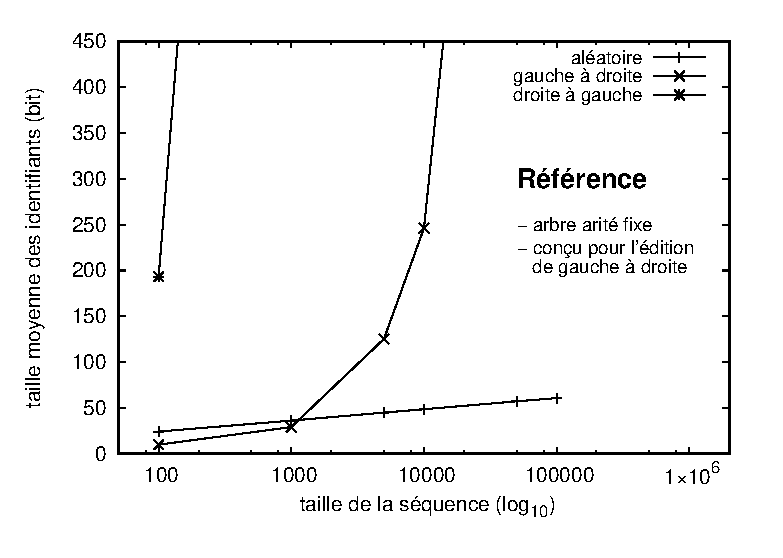
\includegraphics[width=1.25\textwidth]{img/replication/logoot.eps}
  \end{minipage}
  \hspace{1.5cm}
  \begin{minipage}{0.45\textwidth}
    \begin{tikzpicture}
      \node[visible on=<2-4>]
      {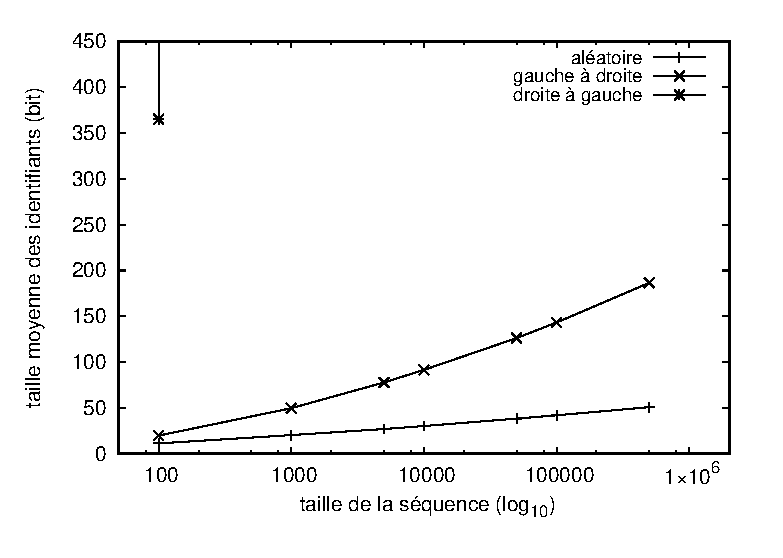
\includegraphics[width=1.25\textwidth]{img/replication/double.eps}};
    \end{tikzpicture}
  \end{minipage}
  
  \hspace{-1cm}
  \begin{minipage}{0.45\textwidth}
    \begin{tikzpicture}
      \node[visible on=<3-4>]
      {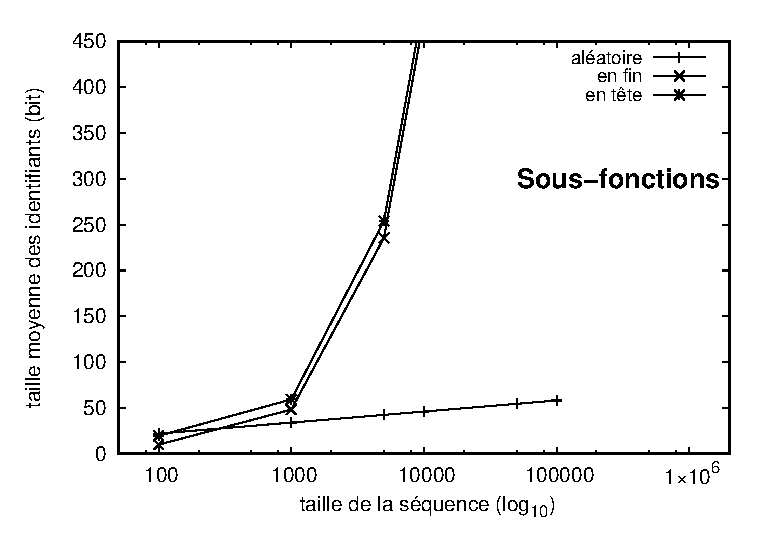
\includegraphics[width=1.25\textwidth]{img/replication/robin.eps}};
    \end{tikzpicture}
  \end{minipage}
  \hspace{1.5cm}
  \begin{minipage}{0.45\textwidth}
    \begin{tikzpicture}
      \node[visible on=<4-4>]
      {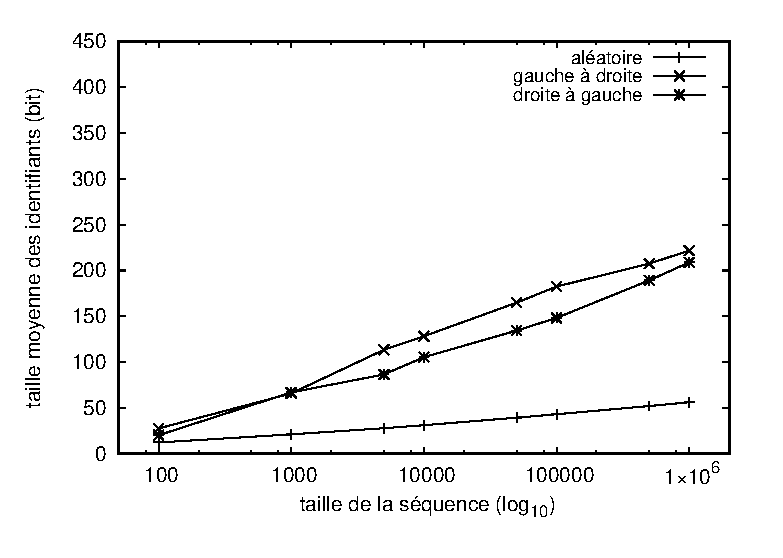
\includegraphics[width=1.25\textwidth]{img/replication/lseq.eps}};
    \end{tikzpicture}
  \end{minipage}

\end{frame}


\begin{frame}{Structure de séquences}{Identifiants sur traces réelles}

  \hspace{-1cm}
  \begin{minipage}{0.45\textwidth}
    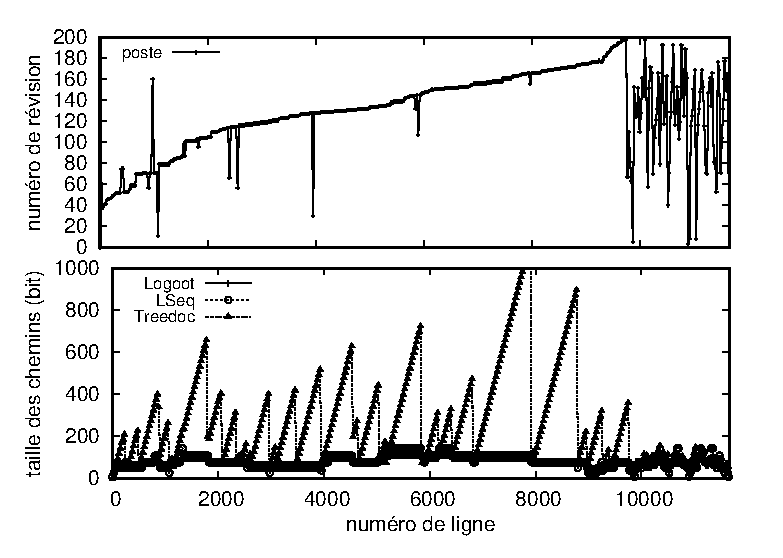
\includegraphics[width=1.29\textwidth]{img/replication/poste.eps}
  \end{minipage}
  \hspace{1.2cm}
  \begin{minipage}{0.45\textwidth}
    \begin{tikzpicture}
      \node[visible on=<2>]
      {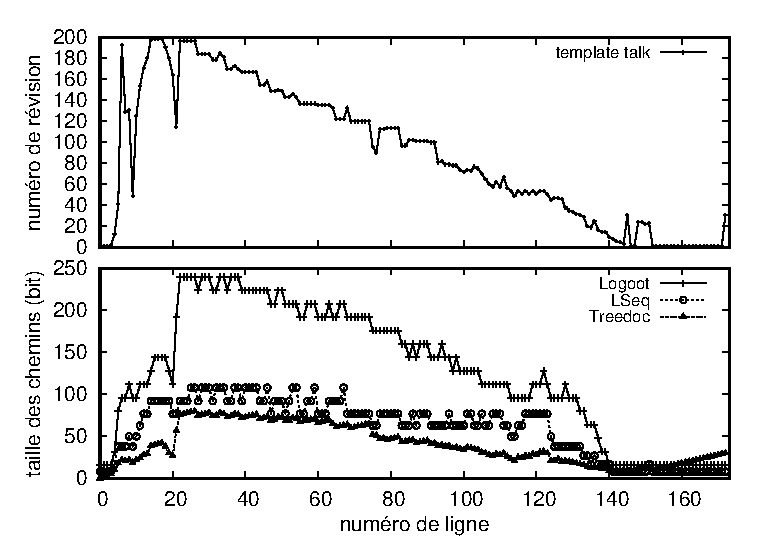
\includegraphics[width=1.29\textwidth]{img/replication/templatetalk.eps}};
    \end{tikzpicture}
  \end{minipage}


\end{frame}


\begin{frame}{Structure de séquences}{Évolution des performances}

  \begin{center}
    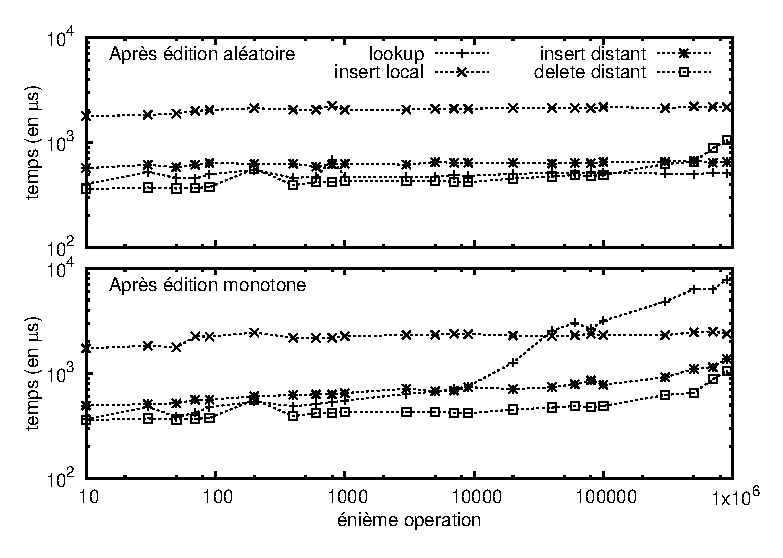
\includegraphics[width=\textwidth]{img/replication/time.eps}
  \end{center}

\end{frame}

\begin{frame}{Structure de séquences}{Effets de la concurrence}
  \vspace{-0.5cm}
  \begin{center}
    \includegraphics[angle=-90, width=\textwidth]{img/replication/latency.eps}
  \end{center}
\end{frame}

\begin{frame}{Structure de séquences}{Conclusion}

%  \begin{itemize}
%  \end{itemize}

\end{frame} %% no begin section right after toc

  \AtBeginSection[]{
    \begin{frame}{Plan}
      \tableofcontents[currentsection]
    \end{frame}
  }
  
  \section{Un protocole d'échantillonnage aléatoire adaptatif}

\begin{frame}{Communication}{Propagation des modifications}

  Préserver la \textbf{cohérence à terme} des documents requière que tous les
  identifiants générés par la structure de séquences soient intégrés par tous
  les éditeurs.
  
  \vspace{0.5cm}
  
  Les éditeurs collaboratifs nécessitent un moyen de \textbf{communiquer} les
  changements effectués sur le document à tous les éditeurs impliqués dans
  l'édition.
  
  \vspace{0.5cm}

  \large
  \begin{itemize}
  \item [$\Rightarrow$] \textbf{Dissémination d'information}
  \end{itemize}
  \vspace{0.5cm}
\end{frame}


\begin{frame}{Communication}{Diffusion épidémique}
  En \textbf{décentralisé}, la diffusion épidémique de messages constitue une
  manière efficace de disséminer l'information. Les messages parviennent à tous
  les pairs sans que ceux-ci ne connaissent tous les membres du réseau.

  \vspace{0.5cm}

  Fonctionnement : chaque pair possède une vue partielle du réseau.
  \begin{enumerate}
  \uncover<2->{\item un pair souhaitant diffuser un message l'envoie à sa vue partielle;}
  \uncover<3->{\item chaque pair recevant un tel message le diffuse à sa vue partielle;}
  \uncover<4->{\item condition d'arrêt : le message a déjà été reçu auparavant.}
  \end{enumerate}

  \begin{minipage}{0.45\textwidth}
    \begin{center}
      \begin{tikzpicture}[scale=1]

\newcommand\X{40pt}
\newcommand\Y{-15pt}

\draw[->] (0*\X, 0*\Y) -- (-5+1*\X,-3*\Y);
\draw[->](0*\X, 0*\Y) -- (-5+1*\X,-0*\Y);
\draw[->] (0*\X, 0*\Y) -- (-5+1*\X, 3*\Y);

% \only<2>\draw[->, very thick] (0*\X, 0*\Y) -- (-5+1*\X,-3*\Y);
% \only<2>\draw[->, very thick](0*\X, 0*\Y) -- (-5+1*\X,-0*\Y);
% \only<2>\draw[->, very thick] (0*\X, 0*\Y) -- (-5+1*\X, 3*\Y);


\draw[->] (1*\X, 3*\Y) -- (-5+2*\X, 4*\Y);
\draw[->] (1*\X, 3*\Y) -- (-5+2*\X, 3*\Y);
\draw[->] (1*\X, 3*\Y) -- (-5+2*\X, 2*\Y);

\draw[->] (1*\X, 0*\Y) -- (-5+2*\X, 1*\Y);
\draw[->] (1*\X, 0*\Y) -- (-5+2*\X, 0*\Y);
\draw[->] (1*\X, 0*\Y) -- (-5+2*\X,-1*\Y);

\draw[->] (1*\X,-3*\Y) -- (-5+2*\X,-2*\Y);
\draw[->] (1*\X,-3*\Y) -- (-5+2*\X,-3*\Y);
\draw[->] (1*\X,-3*\Y) -- (-5+2*\X,-4*\Y);

% \only<3>\draw[->, very thick] (1*\X, 3*\Y) -- (-5+2*\X, 4*\Y);
% \only<3>\draw[->, very thick] (1*\X, 3*\Y) -- (-5+2*\X, 3*\Y);
% \only<3>\draw[->, very thick] (1*\X, 3*\Y) -- (-5+2*\X, 2*\Y);

% \only<3>\draw[->, very thick] (1*\X, 0*\Y) -- (-5+2*\X, 1*\Y);
% \only<3>\draw[->, very thick] (1*\X, 0*\Y) -- (-5+2*\X, 0*\Y);
% \only<3>\draw[->, very thick] (1*\X, 0*\Y) -- (-5+2*\X,-1*\Y);

% \only<3>\draw[->, very thick] (1*\X,-3*\Y) -- (-5+2*\X,-2*\Y);
% \only<3>\draw[->, very thick] (1*\X,-3*\Y) -- (-5+2*\X,-3*\Y);
% \only<3>\draw[->, very thick] (1*\X,-3*\Y) -- (-5+2*\X,-4*\Y);


%\draw[<-, very thick, color=white] (5+1*\X, 5-3*\Y)to[out=90,in=140](-5+2*\X, 5-4*\Y);
%\draw[<-] (5+1*\X, 5-3*\Y)to[out=90,in=140](-5+2*\X, 5-4*\Y);
% \only<4>\draw[<-, very thick] (5+1*\X, 5-3*\Y)to[out=90,in=140](-5+2*\X, 5-4*\Y);
% \only<4>{\draw[fill=white, very thick] ( 2*\X, -4*\Y) node{$e_a$} +(-5pt,-5pt) rectangle +(5pt,5pt);}

%% ea --- ec
\draw[->](2*\X, -4*\Y) -- (3*\X, 5-4*\Y);
\draw[->](2*\X, -4*\Y) -- (3*\X, -5-4*\Y);
\draw[->](2*\X, -4*\Y) -- (3*\X, -0-4*\Y);
%\draw[->](2*\X, -4*\Y) -- (3*\X,  5-4*\Y);

\draw[->](2*\X, -3*\Y) -- (3*\X, -5-3*\Y);
\draw[->](2*\X, -3*\Y) -- (3*\X, -0-3*\Y);
\draw[->](2*\X, -3*\Y) -- (3*\X,  5-3*\Y);

\draw[->](2*\X, -2*\Y) -- (3*\X, -5-2*\Y);
\draw[->](2*\X, -2*\Y) -- (3*\X, -0-2*\Y);
\draw[->](2*\X, -2*\Y) -- (3*\X,  5-2*\Y);

%% ed --- ef
\draw[->](2*\X, -1*\Y) -- (3*\X, -5-1*\Y);
\draw[->](2*\X, -1*\Y) -- (3*\X, -0-1*\Y);
\draw[->](2*\X, -1*\Y) -- (3*\X,  5-1*\Y);

\draw[->](2*\X, -0*\Y) -- (3*\X, -5-0*\Y);
\draw[->](2*\X, -0*\Y) -- (3*\X, -0-0*\Y);
\draw[->](2*\X, -0*\Y) -- (3*\X,  5-0*\Y);

\draw[->](2*\X, 1*\Y) -- (3*\X, -5+1*\Y);
\draw[->](2*\X, 1*\Y) -- (3*\X, -0+1*\Y);
\draw[->](2*\X, 1*\Y) -- (3*\X,  5+1*\Y);

%% eg --- ei
\draw[->](2*\X, 2*\Y) -- (3*\X, -5+2*\Y);
\draw[->](2*\X, 2*\Y) -- (3*\X, -0+2*\Y);
\draw[->](2*\X, 2*\Y) -- (3*\X,  5+2*\Y);

\draw[->](2*\X, 3*\Y) -- (3*\X, -5+3*\Y);
\draw[->](2*\X, 3*\Y) -- (3*\X, -0+3*\Y);
\draw[->](2*\X, 3*\Y) -- (3*\X,  5+3*\Y);

\draw[->](2*\X, 4*\Y) -- (3*\X, -5+4*\Y);
\draw[->](2*\X, 4*\Y) -- (3*\X, -0+4*\Y);
\draw[->](2*\X, 4*\Y) -- (3*\X,  5+4*\Y);


%% ea --- ec
% \only<4>\draw[->, very thick](2*\X, -4*\Y) -- (3*\X, -5-4*\Y);
% \only<4>\draw[->, very thick](2*\X, -4*\Y) -- (3*\X, -0-4*\Y);
% %\only<4>\draw[->, very thick](2*\X, -4*\Y) -- (3*\X,  5-4*\Y);

% \only<4>\draw[->, very thick](2*\X, -3*\Y) -- (3*\X, -5-3*\Y);
% \only<4>\draw[->, very thick](2*\X, -3*\Y) -- (3*\X, -0-3*\Y);
% \only<4>\draw[->, very thick](2*\X, -3*\Y) -- (3*\X,  5-3*\Y);

% \only<4>\draw[->, very thick](2*\X, -2*\Y) -- (3*\X, -5-2*\Y);
% \only<4>\draw[->, very thick](2*\X, -2*\Y) -- (3*\X, -0-2*\Y);
% \only<4>\draw[->, very thick](2*\X, -2*\Y) -- (3*\X,  5-2*\Y);

% %% ed --- ef
% \only<4>\draw[->, very thick](2*\X, -1*\Y) -- (3*\X, -5-1*\Y);
% \only<4>\draw[->, very thick](2*\X, -1*\Y) -- (3*\X, -0-1*\Y);
% \only<4>\draw[->, very thick](2*\X, -1*\Y) -- (3*\X,  5-1*\Y);

% \only<4>\draw[->, very thick](2*\X, -0*\Y) -- (3*\X, -5-0*\Y);
% \only<4>\draw[->, very thick](2*\X, -0*\Y) -- (3*\X, -0-0*\Y);
% \only<4>\draw[->, very thick](2*\X, -0*\Y) -- (3*\X,  5-0*\Y);

% \only<4>\draw[->, very thick](2*\X, 1*\Y) -- (3*\X, -5+1*\Y);
% \only<4>\draw[->, very thick](2*\X, 1*\Y) -- (3*\X, -0+1*\Y);
% \only<4>\draw[->, very thick](2*\X, 1*\Y) -- (3*\X,  5+1*\Y);

% %% eg --- ei
% \only<4>\draw[->, very thick](2*\X, 2*\Y) -- (3*\X, -5+2*\Y);
% \only<4>\draw[->, very thick](2*\X, 2*\Y) -- (3*\X, -0+2*\Y);
% \only<4>\draw[->, very thick](2*\X, 2*\Y) -- (3*\X,  5+2*\Y);

% \only<4>\draw[->, very thick](2*\X, 3*\Y) -- (3*\X, -5+3*\Y);
% \only<4>\draw[->, very thick](2*\X, 3*\Y) -- (3*\X, -0+3*\Y);
% \only<4>\draw[->, very thick](2*\X, 3*\Y) -- (3*\X,  5+3*\Y);

% \only<4>\draw[->, very thick](2*\X, 4*\Y) -- (3*\X, -5+4*\Y);
% \only<4>\draw[->, very thick](2*\X, 4*\Y) -- (3*\X, -0+4*\Y);
% \only<4>\draw[->, very thick](2*\X, 4*\Y) -- (3*\X,  5+4*\Y);



\draw[fill=white] ( 0*\X, 0*\Y) node{$e$} +(-5pt,-5pt) rectangle +(5pt,5pt);
% \only<2>{\draw[fill=white, very thick] ( 0*\X, 0*\Y) node{$e$} +(-5pt,-5pt) rectangle +(5pt,5pt);}

\draw[fill=white] ( 1*\X,-3*\Y) node{$e_1$} +(-5pt,-5pt) rectangle +(5pt,5pt);
\draw[fill=white] ( 1*\X, 0*\Y) node{$e_2$} +(-5pt,-5pt) rectangle +(5pt,5pt);
\draw[fill=white] ( 1*\X, 3*\Y) node{$e_3$} +(-5pt,-5pt) rectangle +(5pt,5pt);

% \only<3>{\draw[fill=white, very thick] ( 1*\X,-3*\Y) node{$e_1$} +(-5pt,-5pt) rectangle +(5pt,5pt);}
% \only<3>{\draw[fill=white, very thick] ( 1*\X, 0*\Y) node{$e_2$} +(-5pt,-5pt) rectangle +(5pt,5pt);}
% \only<3>{\draw[fill=white, very thick] ( 1*\X, 3*\Y) node{$e_3$} +(-5pt,-5pt) rectangle +(5pt,5pt);}


\draw[fill=white] ( 2*\X, -4*\Y) node{$e_a$} +(-5pt,-5pt) rectangle +(5pt,5pt);
\draw[fill=white] ( 2*\X, -3*\Y) node{$e_b$} +(-5pt,-5pt) rectangle +(5pt,5pt);
\draw[fill=white] ( 2*\X, -2*\Y) node{$e_c$} +(-5pt,-5pt) rectangle +(5pt,5pt);

\draw[fill=white] ( 2*\X, -1*\Y) node{$e_d$} +(-5pt,-5pt) rectangle +(5pt,5pt);
\draw[fill=white] ( 2*\X,  0*\Y) node{$e_e$} +(-5pt,-5pt) rectangle +(5pt,5pt);
\draw[fill=white] ( 2*\X,  1*\Y) node{$e_f$} +(-5pt,-5pt) rectangle +(5pt,5pt);

\draw[fill=white] ( 2*\X,  2*\Y) node{$e_g$} +(-5pt,-5pt) rectangle +(5pt,5pt);
\draw[fill=white] ( 2*\X,  3*\Y) node{$e_h$} +(-5pt,-5pt) rectangle +(5pt,5pt);
\draw[fill=white] ( 2*\X,  4*\Y) node{$e_i$} +(-5pt,-5pt) rectangle +(5pt,5pt);

% \only<4>{\draw[fill=white, very thick] ( 2*\X, -4*\Y) node{$e_a$} +(-5pt,-5pt) rectangle +(5pt,5pt);}
% \only<4>{\draw[fill=white, very thick] ( 2*\X, -3*\Y) node{$e_b$} +(-5pt,-5pt) rectangle +(5pt,5pt);}
% \only<4>{\draw[fill=white, very thick] ( 2*\X, -2*\Y) node{$e_c$} +(-5pt,-5pt) rectangle +(5pt,5pt);}

% \only<4>{\draw[fill=white, very thick] ( 2*\X, -1*\Y) node{$e_d$} +(-5pt,-5pt) rectangle +(5pt,5pt);}
% \only<4>{\draw[fill=white, very thick] ( 2*\X,  0*\Y) node{$e_e$} +(-5pt,-5pt) rectangle +(5pt,5pt);}
% \only<4>{\draw[fill=white, very thick] ( 2*\X,  1*\Y) node{$e_f$} +(-5pt,-5pt) rectangle +(5pt,5pt);}

% \only<4>{\draw[fill=white, very thick] ( 2*\X,  2*\Y) node{$e_g$} +(-5pt,-5pt) rectangle +(5pt,5pt);}
% \only<4>{\draw[fill=white, very thick] ( 2*\X,  3*\Y) node{$e_h$} +(-5pt,-5pt) rectangle +(5pt,5pt);}
% \only<4>{\draw[fill=white, very thick] ( 2*\X,  4*\Y) node{$e_i$} +(-5pt,-5pt) rectangle +(5pt,5pt);}



\end{tikzpicture}
    \end{center}
  \end{minipage}
  \hfill
  \begin{minipage}{0.53\textwidth}
    \large
    \begin{itemize}
      \uncover<5->{\item [$\Rightarrow$] \textbf{Comment configurer la taille
          des vues partielles et les peupler ?}
      \begin{itemize}
      \item [$\rightarrow$] Protocole d'échantillonnage de pairs
      \end{itemize}}
    \end{itemize}
  \end{minipage}

\end{frame}


% \begin{frame}{Communication}{Contexte Web}
  
%   \begin{minipage}{0.69\textwidth}
%     Le contexte \textbf{Web} pousse à la \textbf{centralisation :}
%     \begin{itemize}
%     \item problèmes de \textbf{confidentialité}, \textbf{censure}, etc.
%     \uncover<2->{\item problèmes de passage à l'échelle, notamment en \textbf{nombre de
%         collaborateurs};}
%     \uncover<3->{\item problèmes de \textbf{résilience} aux pannes.}
%     \end{itemize}
%   \end{minipage}
%   \hfill
%   \begin{minipage}{0.3\textwidth}
%     
\includegraphics[width=0.7\textwidth]{img/www.png}
%   \end{minipage}

%   \vspace{0.75cm}
  

%   \begin{minipage}{0.32\textwidth}
%     \begin{center}
%       \begin{tikzpicture}
%         \node[visible on=<1-3>]
%         {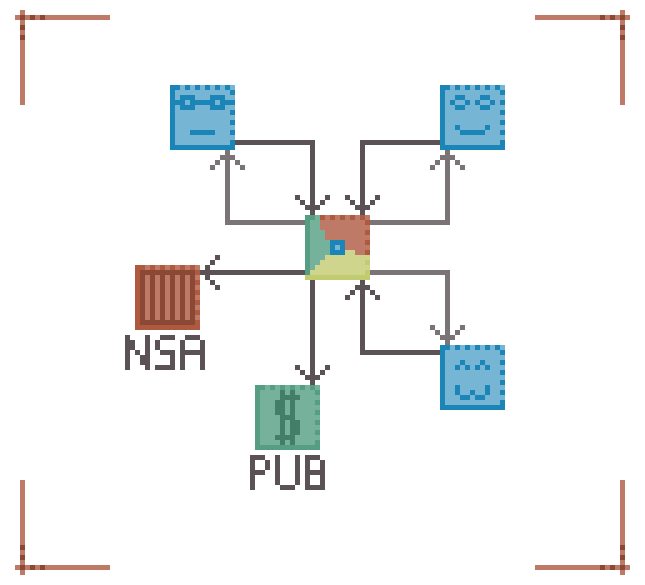
\includegraphics[width=0.95\textwidth]{img/centralizedethicproblems.png}};
%       \end{tikzpicture}
%     \end{center}
%   \end{minipage}
%   \begin{minipage}{0.32\textwidth}
%     \begin{center}
%       \begin{tikzpicture}
%         \node[visible on=<2-3>]
%         {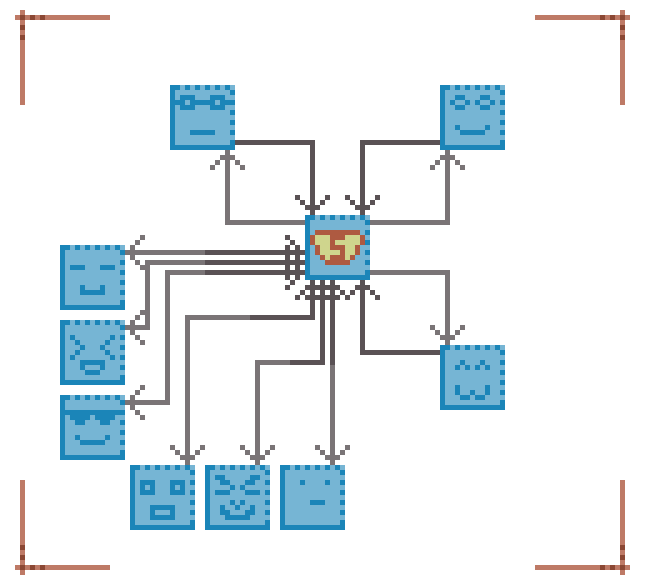
\includegraphics[width=0.95\textwidth]{img/centralizedcpuproblems.png}};
%       \end{tikzpicture}
%     \end{center}
%   \end{minipage}
%   \begin{minipage}{0.32\textwidth}
%     \begin{center}
%       \begin{tikzpicture}
%         \node[visible on=<3-3>]
%         {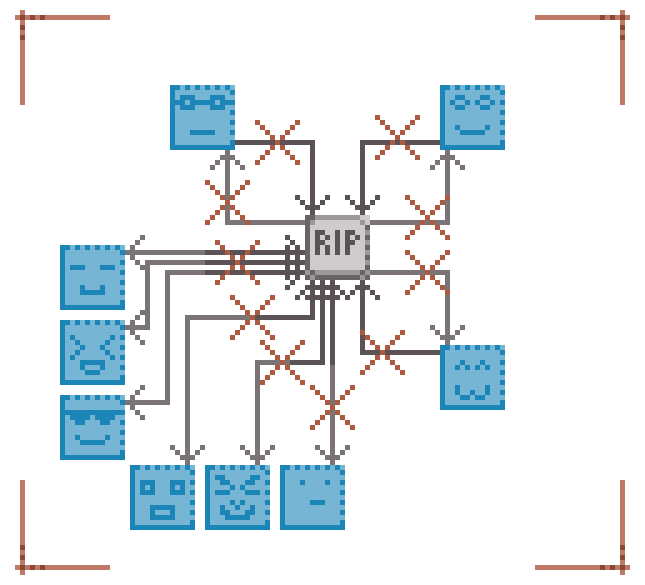
\includegraphics[width=0.95\textwidth]{img/centralizedscalabilityproblems.png}};
%       \end{tikzpicture}        
%     \end{center}
%   \end{minipage}
% \end{frame}


\begin{frame}{Communication}{Possible grâce à WebRTC}


  \begin{minipage}{0.67\textwidth}
    Grâce à WebRTC, les navigateurs Web ne sont plus seulement des clients mais
    aussi des \textbf{serveurs}.
  \end{minipage}
  \hfill
  \begin{minipage}{0.3\textwidth}
    \begin{center}
    
\includegraphics[width=0.6\textwidth]{img/webrtc.png}
    \end{center}
  \end{minipage}
  
  % \vspace{0.5cm}
  \begin{itemize}
  \item \textbf{ni adresses ni routes};
  \item les connexions sont \textbf{coûteuses} et sujettes aux
    \textbf{défaillances};
  \item \textbf{capacités hétérogènes et parfois limitées} des outils de
    navigation;
  \item le contexte Web expose aux \textbf{pics soudains de popularité.}
  \end{itemize}
  
  \vspace{0.5cm}

  \begin{minipage}{0.6\textwidth}
    Pour créer un réseau : 
    \begin{itemize}
      \uncover<2->{\item Un \textbf{serveur sert de médiateur} à la connexion initiale;
      \begin{itemize}
      \item [$\rightarrow$] Au moins 1 aller-retour de messages 
      \end{itemize}}
      \uncover<3->{\item Les pairs \textbf{deviennent des médiateurs} du réseau;}
      \uncover<4>{\item Réseau de trois membres avec connexions directes.}
    \end{itemize}
  \end{minipage}
  \begin{minipage}{0.3\textwidth}
    \begin{center}
      
\begin{tikzpicture}[scale=1.1]

\newcommand\X{40pt};
\newcommand\Y{15pt};

\draw( 1.7*\X, 0); %% spacing
\draw(-1.7*\X, 0); %% spacing

\draw[fill=white,very thick](0*\X, 0*\Y) 
node{serveur de signalement} +(-45pt,-5pt) rectangle +(45pt,5pt);

\small
\only<2>{\draw[->,dashed, very thick](-5 -1*\X, 5-2*\Y) --
node[anchor=east]{1} (-20pt,-5pt);
\draw[<-,dashed, very thick]( 5 -1*\X, 5-2*\Y) --
node[anchor=west]{4} (-10pt,-5pt);

\draw[<-,dashed, very thick](-5pt,  5-3*\Y) --
node[anchor=east]{2}(-5pt,-5pt);
\draw[->,dashed, very thick](5pt , 5-3*\Y) --
node[anchor=west]{3} (5pt,-5pt);}


\draw[fill=white]
(-1*\X,-2*\Y) node{$n_1$} +(-5pt,-5pt) rectangle +(5pt,5pt);
\draw[fill=white]
(0*\X, -3*\Y) node{$n_2$} +(-5pt,-5pt) rectangle +(5pt,5pt);
\draw[fill=white] (1*\X, -2*\Y) node{$n_3$} +(-5pt,-5pt) rectangle +(5pt,5pt);


\small
\only<3>{
\draw[<->, very thick](5-1*\X,-2*\Y)--
node[anchor=south]{1$\rightarrow$}
node[anchor=north]{$\leftarrow$4}(-5pt,-3*\Y);
\draw[<->, very thick](5pt,-3*\Y)--
node[anchor=south]{2$\rightarrow$}
node[anchor=north]{$\leftarrow$3}(-5+1*\X,-2*\Y);
}


\only<4>{
\draw[<->](5-1*\X,-2*\Y)--(-5pt,-3*\Y);
\draw[<->](5pt,-3*\Y)--(-5+1*\X,-2*\Y);
\draw[<->, very thick](5 - 1*\X, 2.5 -2*\Y)--(-5+1*\X, 2.5 -2*\Y);
}


\end{tikzpicture}

    \end{center}
  \end{minipage}
  
  
  % \vspace{0.5cm}
  
  % \large
  % \begin{itemize}
  % \item [$\Rightarrow$] \textbf{Protocole d'échantillonnage de pair adapté à ces
  %     contraintes.}
  % \end{itemize}
  

  
\end{frame}

% \begin{frame}{Communication}{Création de réseau}


% \end{frame}


\begin{frame}{Communication}{Définition du problème}

\begin{problem}
  \label{net:problem:properties}
  Soit $t$ une unité de temps arbitraire, soit $\mathcal{N}^t$ l'ensemble des
  membres non-byzantins du réseau à un instant $t$ et soit $P_i^t$ la vue
  partielle du nœud $n_i \in \mathcal{N}^t$. Un protocole d'échantillonnage
  aléatoire de pairs efficace doit assurer les propriétés suivantes :
  \begin{enumerate}
  \item Taille des vues partielles : \hfill $\forall n_i \in \mathcal{N}^t$,
    $|P_i^t| \approx \mathcal{O}(\ln |\mathcal{N}^t|)$
  \item Établissement de connexion : \hfill $\mathcal{O}(1)$
%  \item \TODO{Convergence}
  \end{enumerate}
\end{problem}

\end{frame}


\begin{frame}{Communication}{État de l'art}

%\vspace{0.5cm}
  
  \begin{itemize}
  \item Vues de taille fixe configurées a priori 
  \end{itemize}
  
  \begin{exampleblock}{Dans un cours en ligne ouvert et massif \ldots}
    \ldots un cours peut commencer avec énormément d'étudiants; rapidement
    perdre en popularité à mesure que l'intérêt des étudiants décline; voir sa
    population croître lorsque les examens finaux arrivent.
  \end{exampleblock}
  
  \vspace{0.5cm}

%  \begin{minipage}{0.37\textwidth}
  \begin{itemize}
  \item Protocole peu adapté au type de connexion WebRTC
  \end{itemize}
  % L'établissement de connexion nécessite au moins 1 aller-retour de message.
%\end{minipage}
%\begin{minipage}{0.61\textwidth}
  \begin{center}
    \begin{tikzpicture}[scale=1.]

\newcommand\X{40pt}
\newcommand\Y{-40pt}

  \draw (-\X, 0); %% align texts

  \small
  \draw (0pt,5pt)node[align=left,anchor=south]{$1_{initie}$\\
    $3_{ach\grave{e}ve}$};
  \draw (2*\X, 5pt)node[anchor=south east]{$2_{accepte}^{Cyclon}$};
  \draw(4*\X,5pt)node[anchor=south]{$2_{accepte}^{Scamp}$};
  \draw (3.5*\X, 0.5*\Y)node{\DARKBLUE{\ldots}};

  \draw[dashed](2*\X,-5pt)--(2*\X,-5+1*\Y);
  \draw[dashed](2*\X, 5pt)--(2*\X, 20pt);

  \normalsize
  \draw[fill=white, thick, draw=darkblue] (0pt, 0pt)
  node{\DARKBLUE{$n_1$}} +(-5pt,-5pt) rectangle +(5pt,5pt);
  \draw[fill=white] (1*\X,\Y) node{$n_2$} +(-5pt,-5pt) rectangle +(5pt,5pt);
  \draw[fill=white] (2*\X, 0pt) node{$n_3$} +(-5pt,-5pt) rectangle +(5pt,5pt);
  \draw[fill=white] (3*\X,\Y) node{$n_4$} +(-5pt,-5pt) rectangle +(5pt,5pt);
  \draw[fill=white, thick, draw=darkblue] (4*\X, 0pt) node{\DARKBLUE{$n_k$}}
  +(-5pt,-5pt) rectangle +(5pt,5pt);


  \draw[->] ( 0pt,-5pt) to[out=-85,in=175] (-5+1*\X,\Y);
  \draw[->, densely dashed] (1*\X, 5+\Y) to[out=95,in=-5] ( 5pt, 0pt);
  \draw     ( 5+1*\X, \Y) to[out=5,in=-95] (2*\X,-5pt);
  \draw[densely dashed] ( -5+2*\X, 0pt) to[out=185,in=85] (1*\X, 5+\Y);
  \draw[->] (2*\X, -5pt) to[out=-85,in=175] (-5+3*\X, \Y);
  \draw[->, densely dashed] (3*\X, 5+\Y) to[out=95,in=-5] (5+2*\X,0pt);
  \draw[->] (5+3*\X, \Y) to[out=5pt,in=-95] (4*\X,-5pt);
  \draw[densely dashed] (-5+4*\X, 0pt) to[out=185,in=85] (3*\X, 5+\Y);
%%  \draw[->, densely dashed] (-70pt, 0pt) -- (-30pt, 0pt); %% u1 -> u4
%%  \draw[->, densely dashed] (-5pt, 30pt) -- (-70pt, 5pt); %% u3 -> u1
%%  \draw[->, densely dashed] (30pt, -5pt) to[out=-85,in=-95](-70pt,-5pt);%%u5 u1

  \small 
  \begin{scope}[shift={(4.5*\X,0pt)}]
    \draw[->](0pt, -12pt)--(10pt, -12pt) node[anchor=west]{Aller};
    \draw[->, densely dashed](0pt, -19pt)--(10pt, -19pt)
    node[anchor=west]{Retour};    
  \end{scope}
  
\end{tikzpicture}
  \end{center}
%\end{minipage}





\end{frame}



\begin{frame}{Communication}{\SPRAY}

  \SPRAY est un protocole d'échantillonnage aléatoire de pairs
  \textbf{adaptatif} supportant le processus complexe d'établissement de
  connexions WebRTC.

  \vspace{0.5cm}

  Chaque pair réagit à des événements et agit périodiquement. Le système
  converge rapidement vers une topologie possédant des propriétés similaires à
  celles des graphes aléatoires.

  \vspace{0.5cm}

  Cycle de vie d'un pair : 
  \begin{enumerate}
  \item \textbf{Rejoindre} le réseau;
  \item \textbf{Rester} dans le réseau;
  \item \textbf{Quitter} le réseau.
  \end{enumerate}

  \large
  \begin{itemize}
  \item [$\Rightarrow$] \textbf{Le nombre de connexions établies doit rester cohérent.}
  \end{itemize}
\end{frame}


\begin{frame}{Communication}{\SPRAY : rejoindre le réseau}

  L'introduction d'un nouveau pair s'accompagne de $1+ \ln {|\mathcal{N}|}$
  connexions.%
  \begin{itemize}
  \item [$\rightarrow$] $|\mathcal{N}|$ pairs implique
    $|\mathcal{N}|\ln |\mathcal{N}|$ connexions.
  \end{itemize}


  \vspace{0.5cm}

  \begin{minipage}{0.6\textwidth}
    \begin{enumerate}[(a)]
    \item Le nouvel arrivant se connecte à un contact ($1$ connexion);
    \uncover<2->{\item Le contact dissémine la nouvelle arrivée aux membres de sa vue;}
    \uncover<3->{\item Chacun de ces voisins établit une connexion
      ($\approx \ln |\mathcal{N}|$ connexions).}
    \end{enumerate}
  \end{minipage}
  \hfill
  \begin{minipage}{0.35\textwidth}
    \begin{center}
      
\begin{tikzpicture}[scale=1.2]

  \newcommand\X{35pt};
  \newcommand\Y{15pt};

%  \draw(-0.75*\X, 0pt); %% positioning
%  \draw( 2.75*\X, 0pt); %% positioning

\only<1>{
  \draw[fill=white, very thick, hide on=1]
  (1*\X,2*\Y) node{$n_6$} +(-5pt,-5pt) rectangle +(5pt,5pt);
  \draw[fill=white, very thick, hide on=1]
  (1*\X,-2*\Y) node{$n_3$} +(-5pt,-5pt) rectangle +(5pt,5pt);
  

  \scriptsize
  \draw[->,dashed,very thick, color=darkblue](5+0*\X, 0*\Y) -- 
  node[anchor=south]{(a)}(-5+ 2*\X, 0*\Y);
  \draw[->] (-5+2*\X, 5pt) -- (5+\X, \Y);
  \draw[->] (-5+2*\X, 5pt) --  (5+\X, 2*\Y);
  \draw[->] (-5+2*\X, -5pt) -- (5+\X, -\Y);
  \draw[->] (-5+2*\X, -5pt) -- (5+\X, -2*\Y);

  \normalsize
  \draw[fill=white, very thick, draw=darkblue]
  (0*\X, 0*\Y) node{\DARKBLUE{$n_1$}} +(-5pt,-5pt) rectangle +(5pt,5pt);
  \draw[fill=white, very thick]
  (2*\X, 0*\Y) node{$n_2$} +(-5pt,-5pt) rectangle +(5pt,5pt);

  \draw[fill=white](1*\X,2*\Y) node{$n_6$} +(-5pt,-5pt) rectangle +(5pt,5pt);
  \draw[fill=white](1*\X,1*\Y) node{$n_5$} +(-5pt,-5pt) rectangle +(5pt,5pt);
  \draw[fill=white](1*\X,-1*\Y) node{$n_4$} +(-5pt,-5pt) rectangle +(5pt,5pt);
  \draw[fill=white](1*\X,-2*\Y) node{$n_3$} +(-5pt,-5pt) rectangle +(5pt,5pt);

}

\only<2>{
  \scriptsize
  \draw[->](5+0*\X, 0*\Y) -- (-5+ 2*\X, 0*\Y);
  \draw[->, very thick, color=darkblue] (-5+2*\X, 5pt) -- (5+\X, \Y);
  \draw[->, very thick, color=darkblue] (-5+2*\X, 5pt) --
  node[anchor=south west]{(b)} (5+\X, 2*\Y);
  \draw[->, very thick, color=darkblue] (-5+2*\X, -5pt) -- (5+\X, -\Y);
  \draw[->, very thick, color=darkblue] (-5+2*\X, -5pt) --
  node[anchor=north west]{(b)}(5+\X, -2*\Y);

  \normalsize
  \draw[fill=white]
  (0*\X, 0*\Y) node{$n_1$} +(-5pt,-5pt) rectangle +(5pt,5pt);
  \draw[fill=white, very thick, draw=darkblue]
  (2*\X, 0*\Y) node{\DARKBLUE{$n_2$}} +(-5pt,-5pt) rectangle +(5pt,5pt);

  \draw[fill=white, very thick]
  (1*\X,2*\Y) node{$n_6$} +(-5pt,-5pt) rectangle +(5pt,5pt);
  \draw[fill=white, very thick]
  (1*\X,1*\Y) node{$n_5$} +(-5pt,-5pt) rectangle +(5pt,5pt);
  \draw[fill=white, very thick]
  (1*\X,-1*\Y) node{$n_4$} +(-5pt,-5pt) rectangle +(5pt,5pt);
  \draw[fill=white, very thick]
  (1*\X,-2*\Y) node{$n_3$} +(-5pt,-5pt) rectangle +(5pt,5pt);
}

\only<3->{

  \scriptsize
  \draw[->](5+0*\X, 0*\Y) -- (-5+ 2*\X, 0*\Y);
  \draw[->] (-5+2*\X, 5pt) -- (5+\X, \Y);
  \draw[->] (-5+2*\X, 5pt) -- (5+\X, 2*\Y);
  \draw[->] (-5+2*\X, -5pt) -- (5+\X, -\Y);
  \draw[->] (-5+2*\X, -5pt) -- (5+\X, -2*\Y);

  \draw[->,dashed, very thick, color=darkblue](-5+\X, 2*\Y) --
  node[anchor=south east]{(c)} ( 5pt,5pt);
  \draw[->,dashed, very thick, color=darkblue](-5+\X, 1*\Y) -- ( 5pt,5pt);
  \draw[->,dashed, very thick, color=darkblue](-5+\X, -1*\Y) -- ( 5pt,-5pt);
  \draw[->,dashed, very thick, color=darkblue](-5+\X, -2*\Y) --
  node[anchor=north east]{(c)}( 5pt,-5pt);

  \normalsize
  \draw[fill=white, very thick]
  (0*\X, 0*\Y) node{$n_1$} +(-5pt,-5pt) rectangle +(5pt,5pt);
  \draw[fill=white]
  (2*\X, 0*\Y) node{$n_2$} +(-5pt,-5pt) rectangle +(5pt,5pt);

  \draw[fill=white, very thick, draw=darkblue]
  (1*\X,2*\Y) node{\DARKBLUE{$n_6$}} +(-5pt,-5pt) rectangle +(5pt,5pt);
  \draw[fill=white, very thick, draw=darkblue]
  (1*\X,1*\Y) node{\DARKBLUE{$n_5$}} +(-5pt,-5pt) rectangle +(5pt,5pt);
  \draw[fill=white, very thick, draw=darkblue]
  (1*\X,-1*\Y) node{\DARKBLUE{$n_4$}} +(-5pt,-5pt) rectangle +(5pt,5pt);
  \draw[fill=white, very thick, draw=darkblue]
  (1*\X,-2*\Y) node{\DARKBLUE{$n_3$}} +(-5pt,-5pt) rectangle +(5pt,5pt);
}


\end{tikzpicture}
    \end{center}
  \end{minipage}
  
  \vspace{1cm}
  
  \large
  \begin{itemize}
  \uncover<4->{\item [$\Rightarrow$] \textbf{Les vues partielles sont déséquilibrées}}
  \end{itemize}

\end{frame}

\begin{frame}{Communication}{\SPRAY : échanges périodiques}
 
  Les échanges périodiques mélangent les vues partielles. Le nombre de
  connexions n'augmente ni ne diminue.
 
  \vspace{0.5cm}

  \begin{minipage}{0.6\textwidth}
    \begin{enumerate}[(a)]
    \item Initiation du mélange périodique. Le pair devient médiateur entre
      $\lceil P \div 2 \rceil - 1$ voisins aléatoires et le pair choisi pour le
      mélange. 
    \uncover<2->{\item En réponse, le pair choisi devient médiateur entre
      $\lceil P\div 2 \rceil$ voisins et le pair initiateur;}
    \uncover<3->{\item Le pair initiateur reçoit la réponse et établit ses 
      connexions grâce au pair choisi.}
    \end{enumerate}
  \end{minipage}
  \begin{minipage}{0.37\textwidth}
    \begin{center}
      
\begin{tikzpicture}[scale=1.1]

  \newcommand\X{35pt};
  \newcommand\Y{15pt};

  \draw[->, hide on=1-](-5+\X, 5+2*\Y)to[out=120,in=30](-10-2*\Y,5+2*\Y); %% 6 -> 9
\only<1>{
  \draw[->](5+0*\X, 0*\Y) -- (-5+ 2*\X, 0*\Y); %% 1 -> 2
  \draw[->] (-5+2*\X, 5pt) -- (5+\X, \Y);
  \draw[->](2*\X,5pt) -- (5+1*\X, 2*\Y); %% 2 -> 6
  \draw[->] (-5+2*\X, -5pt) -- (5+\X, -\Y);
  \draw[->] (-5+2*\X, -5pt) -- (5+\X, -2*\Y);

  \draw[->,very thick, color=darkblue](-5+\X,2*\Y) -- (0pt,5pt); %% 6 -> 1

  \draw[->](-5+\X, 1*\Y) -- ( 5pt,5pt);
  \draw[->](-5+\X, -1*\Y) -- ( 5pt,-5pt);
  \draw[->](-5+\X, -2*\Y) -- ( 5pt,-5pt);

  \draw[->](-5+\X, 5+2*\Y)to[out=120,in=30](0pt,5+2*\Y); %% 6 -> 7
  \draw[->](-5+\X, 5+2*\Y)to[out=120,in=30](-5-\Y ,5+2*\Y); %% 6 -> 8
  \draw[->](-5+\X, 5+2*\Y)to[out=120,in=30](-10-2*\Y,5+2*\Y); %% 6 -> 9

  \normalsize
  \draw[fill=white, very thick]
  (0*\X, 0*\Y) node{$n_1$} +(-5pt,-5pt) rectangle +(5pt,5pt);
  \draw[fill=white](2*\X, 0*\Y) node{$n_2$} +(-5pt,-5pt) rectangle +(5pt,5pt);

  \draw[fill=white,very thick, draw=darkblue]
  (1*\X,2*\Y) node{\DARKBLUE{$n_6$}} +(-5pt,-5pt) rectangle +(5pt,5pt);
  \draw[fill=white](1*\X,1*\Y) node{$n_5$} +(-5pt,-5pt) rectangle +(5pt,5pt);
  \draw[fill=white](1*\X,-1*\Y) node{$n_4$} +(-5pt,-5pt) rectangle +(5pt,5pt);
  \draw[fill=white](1*\X,-2*\Y) node{$n_3$} +(-5pt,-5pt) rectangle +(5pt,5pt);

  \draw[fill=white]( 0*\X,2*\Y)
  node{$n_7$} +(-5pt,-5pt) rectangle +(5pt,5pt);
  \draw[fill=white](-5+-\Y,2*\Y)node{$n_8$} +(-5pt,-5pt) rectangle +(5pt,5pt);
  \draw[fill=white, draw=darkblue](-10+-2*\Y,2*\Y)
  node{\DARKBLUE{$n_9$}} +(-5pt,-5pt) rectangle +(5pt,5pt);
}

\only<2>{
  \draw[->](5+0*\X, 0*\Y) -- (-5+ 2*\X, 0*\Y); %% 1 -> 2
  \draw[->] (-5+2*\X, 5pt) -- (5+\X, \Y);
  \draw[->](2*\X,5pt) -- (5+1*\X, 2*\Y); %% 2 -> 6
  \draw[->] (-5+2*\X, -5pt) -- (5+\X, -\Y);
  \draw[->] (-5+2*\X, -5pt) -- (5+\X, -2*\Y);

  \draw[->,dashed, very thick, color=darkblue](0pt,5pt)--(-5+\X, 2*\Y); %% 1 -> 6

  \draw[->](-5+\X, 1*\Y) -- ( 5pt,5pt);
  \draw[->](-5+\X, -1*\Y) -- ( 5pt,-5pt);
  \draw[->](-5+\X, -2*\Y) -- ( 5pt,-5pt);

  \draw[->](-5+\X, 5+2*\Y)to[out=120,in=30](0pt,5+2*\Y); %% 6 -> 7
  \draw[->](-5+\X, 5+2*\Y)to[out=120,in=30](-5-\Y ,5+2*\Y); %% 6 -> 8
  
  \draw[->,dashed, very thick, color=darkblue](-5pt,5pt)--(-10-2*\Y,-5+2*\Y); %% 1 -> 9

  \normalsize
  \draw[fill=white, very thick]
  (0*\X, 0*\Y) node{$n_1$} +(-5pt,-5pt) rectangle +(5pt,5pt);
  \draw[fill=white, draw=darkblue](2*\X, 0*\Y)
  node{\DARKBLUE{$n_2$}} +(-5pt,-5pt) rectangle +(5pt,5pt);

  \draw[fill=white,very thick]
  (1*\X,2*\Y) node{$n_6$} +(-5pt,-5pt) rectangle +(5pt,5pt);
  \draw[fill=white](1*\X,1*\Y) node{$n_5$} +(-5pt,-5pt) rectangle +(5pt,5pt);
  \draw[fill=white](1*\X,-1*\Y) node{$n_4$} +(-5pt,-5pt) rectangle +(5pt,5pt);
  \draw[fill=white](1*\X,-2*\Y) node{$n_3$} +(-5pt,-5pt) rectangle +(5pt,5pt);

  \draw[fill=white]( 0*\X,2*\Y)
  node{$n_7$} +(-5pt,-5pt) rectangle +(5pt,5pt);
  \draw[fill=white](-5+-\Y,2*\Y)node{$n_8$} +(-5pt,-5pt) rectangle +(5pt,5pt);
  \draw[fill=white](-10+-2*\Y,2*\Y) node{$n_9$} +(-5pt,-5pt) rectangle +(5pt,5pt);
}


\only<3->{
  \draw[->] (-5+2*\X, 5pt) -- (5+\X, \Y);
  \draw[->,dashed, very thick, color=darkblue]
  (5+\X, 2*\Y)to[out=-20,in=110](2*\X, 5pt); %% 6 -> 2
  \draw[->](2*\X,5pt)to[out=160,in=-70](5+1*\X, 2*\Y); %% 2 -> 6
  \draw[->] (-5+2*\X, -5pt) -- (5+\X, -\Y);
  \draw[->] (-5+2*\X, -5pt) -- (5+\X, -2*\Y);

  \draw[->](0pt,5pt)--(-5+\X, 2*\Y); %% 1 -> 6

  \draw[->](-5+\X, 1*\Y) -- ( 5pt,5pt);
  \draw[->](-5+\X, -1*\Y) -- ( 5pt,-5pt);
  \draw[->](-5+\X, -2*\Y) -- ( 5pt,-5pt);

  \draw[->](-5+\X, 5+2*\Y)to[out=120,in=30](0pt,5+2*\Y); %% 6 -> 7
  \draw[->](-5+\X, 5+2*\Y)to[out=120,in=30](-5-\Y ,5+2*\Y); %% 6 -> 8
  
  \draw[->](-5pt,5pt)--(-10-2*\Y,-5+2*\Y); %% 1 -> 9

  \normalsize
  \draw[fill=white]
  (0*\X, 0*\Y) node{$n_1$} +(-5pt,-5pt) rectangle +(5pt,5pt);
  \draw[fill=white](2*\X, 0*\Y) node{$n_2$} +(-5pt,-5pt) rectangle +(5pt,5pt);

  \draw[fill=white,very thick]
  (1*\X,2*\Y) node{$n_6$} +(-5pt,-5pt) rectangle +(5pt,5pt);
  \draw[fill=white](1*\X,1*\Y) node{$n_5$} +(-5pt,-5pt) rectangle +(5pt,5pt);
  \draw[fill=white](1*\X,-1*\Y) node{$n_4$} +(-5pt,-5pt) rectangle +(5pt,5pt);
  \draw[fill=white](1*\X,-2*\Y) node{$n_3$} +(-5pt,-5pt) rectangle +(5pt,5pt);

  \draw[fill=white]( 0*\X,2*\Y)
  node{$n_7$} +(-5pt,-5pt) rectangle +(5pt,5pt);
  \draw[fill=white](-5+-\Y,2*\Y)node{$n_8$} +(-5pt,-5pt) rectangle +(5pt,5pt);
  \draw[fill=white](-10+-2*\Y,2*\Y) node{$n_9$} +(-5pt,-5pt) rectangle +(5pt,5pt);
}

\end{tikzpicture}
    \end{center}
  \end{minipage}


  \vspace{0.5cm}
  \large
  \begin{itemize}
  \uncover<4->{\item [$\Rightarrow$]
    \textbf{Équilibre rapidement la taille des vues partielles;}}
  \uncover<4->{\item [$\Rightarrow$] \textbf{Disperse les connexions.}}
  \end{itemize}
  
\end{frame}

\begin{frame}{Communication}{\SPRAY : quitter le réseau}

  Le départ d'un pair engendre la suppression de $1+\ln|\mathcal{N}|$ connexions.

  \vspace{0.5cm}

  \begin{minipage}{0.6\textwidth}
    \begin{enumerate}[(a)]
    \item Un pair quitte le réseau ou tombe en panne;
    \uncover<2->{\item Les pairs ayant une connexion vers lui s'aperçoivent de sa disparition;}
    \uncover<3->{\item Ces pairs ajoutent de manière probabiliste des doublons.}
    \end{enumerate}
  \end{minipage}
  \hfill
  \begin{minipage}{0.37\textwidth}
    \begin{center}
      
\begin{tikzpicture}[scale=1.1]

  \newcommand\X{35pt};
  \newcommand\Y{15pt};

\draw[fill=white, very thick, draw=darkblue, hide on=1-]
(1*\X,-2*\Y) node{\DARKBLUE{$n_3$}} +(-5pt,-5pt) rectangle +(5pt,5pt);


\only<1>{
  \large
  \draw[->](-5+\X, 1*\Y) --node{$\times$} ( 5pt,5pt);
  \draw[->](-5+\X, -1*\Y) --node{$\times$} ( 5pt,-5pt);
  \draw[->](-5+\X, -2*\Y) --node{$\times$} ( 5pt,-5pt);

  \draw[->, color=darkblue](-5pt,5pt)--
  node{\DARKBLUE{$\times$}}(-10-2*\Y,-5+2*\Y); %% 1 -> 9
  \draw[->, color=darkblue](-5pt,5pt)--
  node{\DARKBLUE{$\times$}}(-5-1*\Y,-5+2*\Y); %% 1 ->8 
  \draw[->, color=darkblue](-5pt,5pt)--
  node{\DARKBLUE{$\times$}}(0pt,-5+2*\Y); %% 1 -> 7
  \draw[->, color=darkblue](-5pt,5pt)--
  node{\DARKBLUE{$\times$}}(-5+\X,-5+2*\Y); %% 1 -> 6

  \normalsize
  \draw[->](5+ 1*\X, 5+ 1*\Y)--(-5+2*\X, 2*\Y); %% 5 -> 14
  \draw[->](5+1*\X,  1*\Y)--(-5+2*\X, 1*\Y); %% 5 -> 13 
  
  \draw[->](5+\X, 5-\Y) -- (-5+2*\X,0pt); %% 4 -> 12
  \draw[->](5+\X, -\Y) -- (-5+2*\X, -\Y); %% 4 -> 11
  
  \draw[->](5+\X, -2*\Y) -- (-5+2*\X, -2*\Y);
  
  \small
  \draw[fill=white,very thick, draw=darkblue]
  (0*\X, 0*\Y) node{\DARKBLUE{$n_1$}} +(-5pt,-5pt) rectangle +(5pt,5pt);
  \draw[thick, color=darkblue] (-5pt,-5pt) -- (5pt,5pt);
  \draw[thick, color=darkblue] (-5pt, 5pt) -- (5pt,-5pt);
  
  \draw[fill=white]
  (1*\X,1*\Y) node{$n_5$} +(-5pt,-5pt) rectangle +(5pt,5pt);
  \draw[fill=white]
  (1*\X,-1*\Y) node{$n_4$} +(-5pt,-5pt) rectangle +(5pt,5pt);
  \draw[fill=white]
  (1*\X,-2*\Y) node{$n_3$} +(-5pt,-5pt) rectangle +(5pt,5pt);

  \draw[fill=white](\X,2*\Y) node{$n_6$} +(-5pt,-5pt) rectangle +(5pt,5pt);

  \draw[fill=white]( 0*\X,2*\Y)
  node{$n_7$} +(-5pt,-5pt) rectangle +(5pt,5pt);
  \draw[fill=white](-5+-\Y,2*\Y)node{$n_8$} +(-5pt,-5pt) rectangle +(5pt,5pt);
  \draw[fill=white](-10+-2*\Y,2*\Y) node{$n_9$} +(-5pt,-5pt) rectangle +(5pt,5pt);
  
  \draw[fill=white](2*\X,2*\Y)node{$n_{14}$} +(-5pt,-5pt) rectangle +(5pt,5pt);
  \draw[fill=white](2*\X,1*\Y)node{$n_{13}$} +(-5pt,-5pt) rectangle +(5pt,5pt);
  \draw[fill=white](2*\X,0*\Y)node{$n_{12}$} +(-5pt,-5pt) rectangle +(5pt,5pt);
  \draw[fill=white](2*\X,-1*\Y)node{$n_{11}$}+(-5pt,-5pt) rectangle +(5pt,5pt);
  \draw[fill=white](2*\X,-2*\Y)node{$n_{10}$}+(-5pt,-5pt) rectangle +(5pt,5pt);

}


\only<2>{

  \large
  \draw[->, very thick, color=darkblue](-5+\X, 1*\Y) --
  node{\DARKBLUE{$\times$}} ( 5pt,5pt);
  \draw[->, very thick, color=darkblue](-5+\X, -1*\Y) --
  node{\DARKBLUE{$\times$}} ( 5pt,-5pt);
  \draw[->, very thick, color=darkblue](-5+\X, -2*\Y) --
  node{\DARKBLUE{$\times$}} ( 5pt,-5pt);

  \normalsize

  \draw[->](5+ 1*\X, 5+ 1*\Y)--(-5+2*\X, 2*\Y); %% 5 -> 14
  \draw[->](  5+1*\X, 1*\Y)--(-5+2*\X, 1*\Y); %% 5 -> 13 (v)
  
  \draw[->](5+\X, 5-\Y) -- (-5+2*\X,0pt); %% 4 -> 12
  \draw[->](5+\X, -\Y) -- (-5+2*\X, -\Y); %% 4 -> 11
  
  \draw[->](5+\X, -2*\Y) -- (-5+2*\X, -2*\Y);
  
  \small
  \draw[fill=white]
  (0*\X, 0*\Y) node{$n_1$} +(-5pt,-5pt) rectangle +(5pt,5pt);
  \draw (-5pt,-5pt) -- (5pt,5pt);
  \draw (-5pt, 5pt) -- (5pt,-5pt);
  
  \draw[fill=white, very thick, draw=darkblue]
  (1*\X,1*\Y) node{\DARKBLUE{$n_5$}} +(-5pt,-5pt) rectangle +(5pt,5pt);
  \draw[fill=white, very thick, draw=darkblue]
  (1*\X,-1*\Y) node{\DARKBLUE{$n_4$}} +(-5pt,-5pt) rectangle +(5pt,5pt);
  \draw[fill=white, very thick, draw=darkblue]
  (1*\X,-2*\Y) node{\DARKBLUE{$n_3$}} +(-5pt,-5pt) rectangle +(5pt,5pt);

  \draw[fill=white](\X,2*\Y) node{$n_6$} +(-5pt,-5pt) rectangle +(5pt,5pt);

  \draw[fill=white]( 0*\X,2*\Y)
  node{$n_7$} +(-5pt,-5pt) rectangle +(5pt,5pt);
  \draw[fill=white](-5+-\Y,2*\Y)node{$n_8$} +(-5pt,-5pt) rectangle +(5pt,5pt);
  \draw[fill=white](-10+-2*\Y,2*\Y) node{$n_9$} +(-5pt,-5pt) rectangle +(5pt,5pt);
  
  \draw[fill=white](2*\X,2*\Y)node{$n_{14}$} +(-5pt,-5pt) rectangle +(5pt,5pt);
  \draw[fill=white](2*\X,1*\Y)node{$n_{13}$} +(-5pt,-5pt) rectangle +(5pt,5pt);
  \draw[fill=white](2*\X,0*\Y)node{$n_{12}$} +(-5pt,-5pt) rectangle +(5pt,5pt);
  \draw[fill=white](2*\X,-1*\Y)node{$n_{11}$}+(-5pt,-5pt) rectangle +(5pt,5pt);
  \draw[fill=white](2*\X,-2*\Y)node{$n_{10}$}+(-5pt,-5pt) rectangle +(5pt,5pt);
}

\only<3->{

  \draw[->](5+ 1*\X, 5+ 1*\Y)--(-5+2*\X, 2*\Y); %% 5 -> 14
  \draw[->](5+1*\X, 2.5+ 1*\Y)--(-5+2*\X, 2.5+ 1*\Y); %% 5 -> 13 (^)
  \draw[->,dashed, very thick, color=darkblue]
  (  5+1*\X,-2.5+1*\Y)--(-5+2*\X,-2.5+1*\Y); %% 5 -> 13 (v)
  
  \draw[->](5+\X, 5-\Y) -- (-5+2*\X,0pt); %% 4 -> 12
  \draw[->](5+\X, -\Y) -- (-5+2*\X, -\Y); %% 4 -> 11
  
  \draw[->](5+\X, 2.5-2*\Y) -- (-5+2*\X, 2.5-2*\Y);
  \draw[->,dashed, very thick, color=darkblue](5+\X, -2.5-2*\Y) -- (-5+2*\X , -2.5-2*\Y);
  
  \small
  \draw[fill=white]
  (0*\X, 0*\Y) node{$n_1$} +(-5pt,-5pt) rectangle +(5pt,5pt);
  \draw (-5pt,-5pt) -- (5pt,5pt);
  \draw (-5pt, 5pt) -- (5pt,-5pt);
  
  \draw[fill=white, very thick]
  (1*\X,1*\Y) node{$n_5$} +(-5pt,-5pt) rectangle +(5pt,5pt);
  \draw[fill=white, very thick]
  (1*\X,-1*\Y) node{$n_4$} +(-5pt,-5pt) rectangle +(5pt,5pt);
  \draw[fill=white, very thick]
  (1*\X,-2*\Y) node{$n_3$} +(-5pt,-5pt) rectangle +(5pt,5pt);

  \draw[fill=white](\X,2*\Y) node{$n_6$} +(-5pt,-5pt) rectangle +(5pt,5pt);

  \draw[fill=white]( 0*\X,2*\Y)
  node{$n_7$} +(-5pt,-5pt) rectangle +(5pt,5pt);
  \draw[fill=white](-5+-\Y,2*\Y)node{$n_8$} +(-5pt,-5pt) rectangle +(5pt,5pt);
  \draw[fill=white](-10+-2*\Y,2*\Y) node{$n_9$} +(-5pt,-5pt) rectangle +(5pt,5pt);
  
  \draw[fill=white](2*\X,2*\Y)node{$n_{14}$} +(-5pt,-5pt) rectangle +(5pt,5pt);
  \draw[fill=white](2*\X,1*\Y)node{$n_{13}$} +(-5pt,-5pt) rectangle +(5pt,5pt);
  \draw[fill=white](2*\X,0*\Y)node{$n_{12}$} +(-5pt,-5pt) rectangle +(5pt,5pt);
  \draw[fill=white](2*\X,-1*\Y)node{$n_{11}$}+(-5pt,-5pt) rectangle +(5pt,5pt);
  \draw[fill=white](2*\X,-2*\Y)node{$n_{10}$}+(-5pt,-5pt) rectangle +(5pt,5pt);

}

\end{tikzpicture}
    \end{center}
  \end{minipage}

  \vspace{1cm}
  \large
  \begin{itemize}
  \uncover<4->{\item[$\Rightarrow$] \textbf{Présence de doublons assure la cohérence du nombre de connexions.}
  \begin{itemize}
  \item [$\rightarrow$] Mais impacte négativement les propriétés du réseau.
  \end{itemize}}
  \end{itemize}
 
\end{frame}


\begin{frame}{Communication}{Expérimentations}

  Simulations \PEERSIM.

  \vspace{0.5cm}

  \begin{itemize}
  \item \CYCLON : vue partielle dont la taille est configurée \textit{a priori};
%  \item \SCAMP : vue partielle dont la taille s'ajuste au réseau;
  \item \SPRAY : vue partielles dont la taille s'ajuste au réseau et adapté au
    contexte Web.
  \end{itemize}

%\end{frame}

%\begin{frame}{Communication}{Résultats attendus}
  
  \vspace{0.5cm}


  Résultats attendus :
  \begin{itemize}
  \item Convergence rapide vers un réseau possédant des propriétés similaires à
    celles des graphes aléatoires;
  \item Les doublons sont peu nombreux et n'impactent pas significativement les
    propriétés du réseau;
  \item Les protocoles basés sur \SPRAY bénéficient de son adaptativité.
  \end{itemize}

\end{frame}

\begin{frame}{Communication}{Coefficient d'agglomération diminue rapidement}
  \hspace{-1cm}
  \begin{minipage}{0.47\textwidth}
    \begin{center}
      \includegraphics[width=1.23\textwidth]{img/network/cycloncluster.eps}
    \end{center}
  \end{minipage}
  \hfill
  \begin{minipage}{0.47\textwidth}
      \includegraphics[width=1.23\textwidth]{img/network/spraycluster.eps}
  \end{minipage}

  \vspace{0.5cm}

  \begin{itemize}
  \item \CYCLON configuré avec
    \begin{itemize}
    \item  $\ln(1000) \approx 7$ voisins et
    \item mélange de $3$ voisins.
    \end{itemize}
  \end{itemize}

\end{frame}


\begin{frame}{Communication}{L'information se propage rapidement}
  \begin{center}
    \includegraphics[width=1\textwidth]{img/network/avgpath.eps}
  \end{center}
\end{frame}

\begin{frame}{Communication}{La charge est équilibrée}
  \begin{center}
    \includegraphics[width=1\textwidth]{img/network/histo.eps}
  \end{center}
\end{frame}


\begin{frame}{Communication}{Les vues partielles s'adaptent}
  \hspace{-1cm}
  \begin{minipage}{0.47\textwidth}
    \begin{center}
      \includegraphics[width=1.23\textwidth]{img/network/churn.eps}
    \end{center}
  \end{minipage}
  \hfill
  \begin{minipage}{0.47\textwidth}
      \includegraphics[width=1.23\textwidth]{img/network/avgpv.eps}
  \end{minipage}
\end{frame}


\begin{frame}{Communication}{Robuste aux défaillances}
  \begin{center}
    \includegraphics[width=1\textwidth]{img/network/resilience.eps}
  \end{center}
\end{frame}


\begin{frame}{Communication}{Faible taux de doublons}
  \begin{center}
    \includegraphics[width=1\textwidth]{img/network/duplicates.eps}
  \end{center}
\end{frame}


\begin{frame}{Communication}{Cas de la diffusion de messages}
  \begin{algorithm}[H]
    
\small
\algrenewcommand{\algorithmiccomment}[1]{\hskip2em$\rhd$ #1}

\newcommand{\comment}[1]{\hfill $\rhd$ #1}

\newcommand{\LINEFOR}[2]{%
  \algorithmicfor\ {#1}\ \algorithmicdo\ {#2} %
  }

\newcommand{\LINEIFTHEN}[2]{%
  \algorithmicif\ {#1}\ \algorithmicthen\ {#2} %
  }

\newcommand{\INDSTATE}[1][1]{\State\hspace{\algorithmicindent}}

\begin{algorithmic}[1]
  \Function{broadcast}{$m$} \comment{$m$: \emph{message à envoyer}}
  \State \textbf{let} $chosen \leftarrow getPeers(P,\, \DARKBLUE{fanout})$;
  \For{(\DARKBLUE{$n \in chosen$})}
  \State \textsc{sendTo}($n$, 'broadcast', $m$);
  \EndFor
  \EndFunction

  \Statex

  \Function{onBroadcast}{$m$} \comment{$m$: \emph{message reçu}}
  \If {($\DARKBLUE{\neg}$\DARKBLUE{\textsc{alreadyReceived}}$\DARKBLUE{(m)}$)}
  \State \textsc{broadcast}($m$);
  \EndIf
  \EndFunction
\end{algorithmic}

  \end{algorithm}

  \begin{itemize}
  \item \CYCLON 
    \begin{enumerate}
    \item vue partielle de 30 voisins, fanout de $\ln(100)+1\approx 6$;
    \item vue partielle de 30 voisins, fanout de  $\ln(100)+3 \approx 8$.
    \end{enumerate}
  \item \SPRAY
    \begin{enumerate}
    \item vue partielle de $6\cdot\ln|\mathcal{N}|$ voisins,
      fanout de $\ln(|\mathcal{N}|)+1$;
    \item vue partielle de $6\cdot\ln|\mathcal{N}|$ voisins,
      fanout de $\ln(|\mathcal{N}|)+3$;
    \end{enumerate}
  \end{itemize}

%  \vspace{0.5cm}

  \begin{itemize}
  \item[$\rightarrow$] \CYCLON et \SPRAY sont équivalent à 100 pairs
  \end{itemize}
\end{frame}

\begin{frame}{Communication}{Le taux d'erreur reste constant}
  \begin{center}
    \includegraphics[width=1\textwidth]{img/network/hardrate.eps}
  \end{center} 
\end{frame}

\begin{frame}{Communication}{Le pic de popularité est mieux géré}
  \begin{center}
    \includegraphics[width=1\textwidth]{img/network/peak.eps}
  \end{center} 
\end{frame}



\begin{frame}{Communication}{Conclusion}
  
  \begin{itemize}
  \item \SPRAY est un protocole d'échantillonnage aléatoire de pair adaptatif.
  \item \SPRAY est adapté au processus complexe d'établissement de connexion de
    WebRTC.
  \end{itemize}

  \vspace{0.25cm}

  \begin{itemize}
  \item \SPRAY a le désavantage d'utiliser des doublons, mais leur faible
    proportion n'impacte pas les propriétés du réseau.    
  \end{itemize}

  \vspace{0.25cm}

  \begin{itemize}
  \item Les protocoles construits au dessus de \SPRAY bénéficient de cette
    adaptativité.
  \end{itemize}

\end{frame}
  \section{Un éditeur collaboratif temps réel dans les navigateurs}

\begin{frame}
  editor
\end{frame}



  \section{Conclusion et perspectives}

% \begin{frame}{Conclusion}{Éditeur collaboratif Web décentralisé}
  
%   \begin{center}
%     \includegraphics[width=0.85\textwidth]{img/cratescreenshot.png}
%   \end{center}

% \end{frame}


% \begin{frame}{Conclusion}{Architecture}
% %  \hspace{-1cm}

% %  \begin{minipage}{0.47\textwidth}
%     \begin{center}
%       \begin{tikzpicture}[scale=0.8]

\newcommand\X{25pt}
\newcommand\Y{20pt}

\newcommand\LIGHTGRAY{gray!20}
\newcommand\MEDIUMGRAY{gray!40}

\tiny
%% communication
\draw[rounded corners=2mm, color=\MEDIUMGRAY, fill=white](0pt, 0pt)+(-4*\X,-\Y)rectangle+(4*\X,\Y);
\draw(4*\X, \Y)node[anchor=north east]{\textbf{communication}};

\draw[fill=white](-2*\X, -0.25*\Y)
node{dissémination}+(-0.85*\X,-0.5*\Y)rectangle+(0.85*\X,0.5*\Y);
\draw[fill=white, very thick, draw=darkblue]( 0*\X, 0.25*\Y)
node[align=center]{\DARKBLUE{appartenance}}+(-0.85*\X,-0.5*\Y)rectangle+(0.85*\X,0.5*\Y);
\draw[fill=white]( 2*\X, -0.25*\Y)
node{monodiffusion}+(-0.85*\X,-0.5*\Y)rectangle+(0.85*\X,0.5*\Y);

\draw[<-](-0.85*\X, 0.25*\Y)--(-1.15*\X, -0.25*\Y);
\draw[<-](0.85*\X, 0.25*\Y)--(1.15*\X, -0.25*\Y);

%% causality
\draw[rounded corners=2mm, color=\MEDIUMGRAY, fill=\LIGHTGRAY](0pt, -2*\Y)+(-4*\X,-\Y)rectangle+(4*\X,\Y);
\draw(4*\X, -\Y)node[anchor=north east]{\textbf{causalité}};

\draw[fill=\LIGHTGRAY](-2*\X, -2*\Y)
node[align=center]{détection\\[-1mm]des relations\\[-1mm]causales}
+(-1.0*\X,-0.6*\Y)rectangle+(1.0*\X,0.6*\Y);
\tiny
\draw[->, thick](-1.5*\X, -0.75*\Y) -- node[anchor=west]{reçoit}
(-1.5*\X, -1.4*\Y);
\draw[<-, thick](-2.5*\X, -0.75*\Y) -- node[anchor=east]{envoie}
(-2.5*\X, -1.4*\Y);
\tiny
\draw[<->]( 2*\X, -0.75*\Y)--( 1*\X, -2.5*\Y);

%% sequence structure
\draw[rounded corners=2mm, color=\MEDIUMGRAY, fill=white](0pt, -4*\Y)+(-4*\X,-\Y)rectangle+(4*\X,\Y);
\draw(4*\X, -3*\Y)node[anchor=north east, align=right]
{\textbf{structure}\\\textbf{pour}\\\textbf{séquences}};

\draw[fill=white, shading=axis,top color=\LIGHTGRAY, bottom color=white, shading angle=0](1*\X, -3*\Y)
node{anti-entropie}+(-0.95*\X,-0.5*\Y) rectangle +(0.95 *\X, 0.5*\Y);
\draw[fill=white, very thick, draw=darkblue](-2*\X, -4*\Y)
node{\DARKBLUE{réplique}}+(-0.75*\X,-0.5*\Y) rectangle +(0.75 *\X, 0.5*\Y);

\draw[->] (0.05*\X, -2.75*\Y)--(-1*\X,-2*\Y);
\draw[->] (0.05*\X, -3.25*\Y)--(-1.25*\X,-4*\Y);
\tiny
\draw[<-, thick] (-1.5*\X, -3.5*\Y)--node[anchor=west]{délivre}(-1.5*\X, -2.6*\Y);
\draw[->, thick] (-2.5*\X, -3.5*\Y)--node[anchor=east]{décore}(-2.5*\X, -2.6*\Y);
\tiny
%% gui
\draw[rounded corners=2mm, color=\MEDIUMGRAY, fill=\LIGHTGRAY](0pt, -6*\Y)+(-4*\X,-\Y)rectangle+(4*\X,\Y);
\draw(4*\X, -5*\Y)node[anchor=north east, align=right]
{\textbf{interface}\\\textbf{utilisateur}};
\draw[fill=\LIGHTGRAY](0pt,-6*\Y)
node{éditeur web}+(-0.85*\X,-0.5*\Y) rectangle +(0.85 *\X, 0.5*\Y);

%%\draw[<->] (-2*\X, -4.5*\Y) -- (0*\X, -5.5*\Y);
\tiny
\draw[->, thick] (-1.80*\X, -4.5*\Y)--node[anchor=west]{notifie}(-0.85*\X, -5.75*\Y);
\draw[<-, thick] (-2.20*\X, -4.5*\Y)--node[anchor=east]{met à jour}(-0.85*\X, -6.25*\Y);
\tiny
\end{tikzpicture}
%     \end{center}
% %  \end{minipage}
    
%     Le trafic croît 
%     \begin{itemize}
%     \item logarithmiquement par rapport au nombre de collaborateurs grâce à \SPRAY;
%     \item polylogarithmiquement par rapport au nombre d'insertions dans le
%       document grâce à \LSEQ.
%     \end{itemize}

%  \hfill
  % \hspace{0.5cm}
  % \begin{minipage}{0.47\textwidth}
  %   \begin{center}
  %     
\begin{tikzpicture}[scale=1.3]

  \newcommand\X{35pt}
  \newcommand\Y{-35pt}
  
%  \small

%  \draw (-35-2*\X, 30pt);

  
%  \draw[fill=white] (-2*\X, 1.5*\Y) 
%  node{\includegraphics[width=12pt]{img/crateicon.png}};
  % node{$e_9$}; % +(-5pt,-5pt) rectangle +(5pt,5pt);
  % \only<3>{
  %   \draw[<->, densely dashed, color=darkblue, very thick]
  %   (-2*\X, 5+1.5*\Y) -- node[anchor=east]{\DARKBLUE{rejoint}} (-2*\X, -5pt);
  % }
  % \only<4-5>{
  %   \draw[<->, densely dashed, color=darkblue, very thick]
  %   (-2*\X, 5+1.5*\Y) -- (-2*\X, -5pt);
  % }
  % \only<4>{
  %   \draw[->, very thick] (5-2*\X, 10+1.5*\Y) -- (5-2*\X, -10pt);
  %   \draw[->, very thick] (20-2*\X, -10pt) -- (-12pt, \Y);
  % }
  % \only<5>{
  %   \draw[<-, very thick] (5-2*\X, 10+1.5*\Y) -- (5-2*\X, -10pt);
  %   \draw[<-, very thick] (20-2*\X, -10pt) -- (-12pt, \Y);
  % }

  % \only<6->{
  %   \draw[<->, very thick](5-2*\X,1.5*\Y) -- (-5pt, -3+ \Y);
  % }


  % \only<8->{
  %   \draw[<->, very thick](5-2*\X, -3+1.5*\Y ) -- (-5+3*\X ,1*\Y);
  % }

  %   \draw[fill=white] (-2*\X, 0) node{$mediateur_1$} +(-20pt,
  %   -5pt)rectangle+(18pt, 5pt);
  %   \only<2->{
  %   \draw[<->, densely dashed, color=darkblue, very thick]
  %   (20-2*\X, 0) -- node[anchor=south]{\DARKBLUE{partage}} (-5+\X, 0);
  %   \draw[<->, densely dashed, color=darkblue, very thick]
  %   (20-2*\X, -5pt) -- (-5pt, \Y);
  % }
  
  %   \draw[fill=white] (-2*\X, 3*\Y) node{$mediateur_2$} +(-18pt, -5pt)rectangle+(18pt, 5pt);
  % \only<2->{
  %   \draw[<->, densely dashed, color=darkblue] (20-2*\X, 3*\Y) -- (-5+\X, 3*\Y);
  %   \draw[<->, densely dashed, color=darkblue] (20-2*\X, 5+3*\Y) -- (-5pt, 2*\Y);
  % }

  \draw[fill=white] (\X, 0)node{\includegraphics[width=18pt]{img/firefox.png}};
  % node{$e_1$}+(-5pt, -5pt)rectangle+(5pt, 5pt);
  \draw[fill=white] (2*\X, 0)node{\includegraphics[width=18pt]{img/chrome.png}};
  % {$e_2$}+(-5pt, -5pt)rectangle+(5pt, 5pt);
  \draw[fill=white] (3*\X, \Y)node{\includegraphics[width=18pt]{img/chrome.png}};
  % ;{$e_3$}+(-5pt, -5pt)rectangle+(5pt, 5pt);
  \draw[fill=white] (3*\X, 2*\Y)node{\includegraphics[width=18pt]{img/firefox.png}};
  % {$e_4$}+(-5pt, -5pt)rectangle+(5pt, 5pt);
  \draw[fill=white] (2*\X, 3*\Y)node{\includegraphics[width=18pt]{img/chrome.png}};
  % {$e_5$}+(-5pt, -5pt)rectangle+(5pt, 5pt);
  \draw[fill=white] (1*\X, 3*\Y)node{\includegraphics[width=18pt]{img/firefox.png}};
  % {$e_6$}+(-5pt, -5pt)rectangle+(5pt, 5pt);
  \draw[fill=white] (0 , 2*\Y)node{\includegraphics[width=18pt]{img/firefox.png}};
  % {$e_7$}+(-5pt, -5pt)rectangle+(5pt, 5pt);
  % \draw[fill=white] (0 , \Y)+(-55pt, -10pt)rectangle+(5pt, 10pt);
  \draw[fill=white](0,\Y)node{\includegraphics[width=18pt]{img/chrome.png}};
  % {$e_8$}+(-5pt, -5pt)rectangle+(5pt, 5pt);


  \draw[->] (\X, 0)--(\X, 5+3*\Y); %% p1 p6
  \draw[->] (-5+2*\X, 0)--(5+\X, 0); %% p2 p1
  \draw[->] (2*\X, 0) -- (-5+3*\X, \Y); %% p2 p3
  \draw[->] (2*\X, 0) -- (-5+3*\X, 2*\Y); %% p2 p4
  \draw[->] (3*\X, 5+\Y) -- ( 5+2*\X, 0); %% p3 p2
  \draw[->] (3*\X, \Y) -- (5pt, 2*\Y); %% p3 p7
  \draw[->] (3*\X, \Y) -- (2*\X, 5+3*\Y); %% p3 p5
  \draw[->] (3*\X, 2*\Y) -- (5pt, 2*\Y); %% p4 p7
  \draw[->] (3*\X, 2*\Y) -- (5pt, \Y); %% p4 p8
  \draw[->] (2*\X, 3*\Y) -- (\X, -5pt); %% p5 p1
  \draw[->] (5+2*\X, 3*\Y) -- (3*\X, -5+ 2*\Y); %% p5 p4
  \draw[->] (-5+\X, 3*\Y) -- (0pt, -5+2*\Y); %% p6 p7
  \draw[->] (0pt, 2*\Y) -- (-5+3*\X, \Y); %% p7 p3
  \draw[->] (0pt, 2*\Y) -- (\X, -5pt); %% p7 p1
  \draw[->] (0pt, \Y) -- (2*\X, -5pt); %% p8 p2
  \draw[->] (0pt, \Y) -- (\X, 5+3*\Y); %% p8 p6
  \draw[->] (0pt, \Y) -- (-5+3*\X, \Y); %% p8 p3

  \draw[fill=white] (\X, 0)node{\includegraphics[width=12pt]{img/crateicon.png}};
  \draw[fill=white] (2*\X, 0)node{\includegraphics[width=12pt]{img/crateicon.png}};
  \draw[fill=white] (3*\X, \Y)node{\includegraphics[width=12pt]{img/crateicon.png}};
  \draw[fill=white] (3*\X, 2*\Y)node{\includegraphics[width=12pt]{img/crateicon.png}};
  \draw[fill=white] (2*\X, 3*\Y)node{\includegraphics[width=12pt]{img/crateicon.png}};
  \draw[fill=white] (1*\X, 3*\Y)node{\includegraphics[width=12pt]{img/crateicon.png}};
  \draw[fill=white] (0, 2*\Y)node{\includegraphics[width=12pt]{img/crateicon.png}};
  \draw[fill=white] (0, \Y)node{\includegraphics[width=12pt]{img/crateicon.png}};


  \only<2->{
    \draw (0pt, \Y) node{\textbf{A}};
  }

  \only<3>{
    \draw[->, very thick] (0pt, \Y) -- (2*\X, -5pt); %% p8 p2
    \draw[->, very thick] (0pt, \Y) -- (\X, 5+3*\Y); %% p8 p6
    \draw[->, very thick] (0pt, \Y) -- (-5+3*\X, \Y); %% p8 p3

    \draw[fill=white] (0*\X, \Y)node{\includegraphics[width=12pt]{img/crateicon.png}};
    \draw (0pt, \Y) node{\textbf{A}};
  }
  
  \only<3->{
    \draw (2*\X, 0pt) node{\textbf{A}};
    \draw (\X, 3*\Y) node{\textbf{A}};
    \draw (3*\X, \Y) node{\textbf{A}};
  }
  
  \only<4>{
    \draw[->, very thick] (-5+2*\X, 0)--(5+\X, 0); %% p2 p1
    \draw[->, very thick] (2*\X, 0) -- (-5+3*\X, \Y); %% p2 p3
    \draw[->, very thick] (2*\X, 0) -- (-5+3*\X, 2*\Y); %% p2 p4
    \draw (2*\X, 0)node{\includegraphics[width=12pt]{img/crateicon.png}}node{\textbf{A}};
    
    \draw[->, very thick] (-5+\X, 3*\Y) -- (0pt, -5+2*\Y); %% p6 p7
    \draw (\X, 3*\Y)node{\includegraphics[width=12pt]{img/crateicon.png}}node{\textbf{A}};

    \draw[->, very thick] (3*\X, 5+\Y) -- ( 5+2*\X, 0); %% p3 p2
    \draw[->, very thick] (3*\X, \Y) -- (5pt, 2*\Y); %% p3 p7
    \draw[->, very thick] (3*\X, \Y) -- (2*\X, 5+3*\Y); %% p3 p5
    \draw (3*\X, \Y)node{\includegraphics[width=12pt]{img/crateicon.png}}node{\textbf{A}};
  }

  \only<4->{
    \draw (\X, 0) node{\textbf{A}};
    \draw (3*\X, \Y) node{\textbf{A}};
    \draw (3*\X, 2*\Y) node{\textbf{A}};

    \draw (2*\X, 0pt) node{\textbf{A}};
    \draw (0pt, 2*\Y) node{\textbf{A}};
    \draw (2*\X, 3*\Y) node{\textbf{A}};
  }

  \only<5>{
    \draw[->, very thick] (\X, 0)--(\X, 5+3*\Y); %% p1 p6
    \draw (\X, 0)node{\includegraphics[width=12pt]{img/crateicon.png}}node{\textbf{A}};

    \draw[->, very thick] (3*\X, 2*\Y) -- (5pt, 2*\Y); %% p4 p7
    \draw[->, very thick] (3*\X, 2*\Y) -- (5pt, \Y); %% p4 p8
     \draw (3*\X, 2*\Y)node{\includegraphics[width=12pt]{img/crateicon.png}}node{\textbf{A}}; 
    \draw[->, very thick] (2*\X, 3*\Y) -- (\X, -5pt); %% p5 p1
    \draw[->, very thick] (5+2*\X, 3*\Y) -- (3*\X, -5+ 2*\Y); %% p5 p4
    \draw (2*\X, 3*\Y)node{\includegraphics[width=12pt]{img/crateicon.png}}node{\textbf{A}};
    \draw[->, very thick] (0pt, 2*\Y) -- (-5+3*\X, \Y); %% p7 p3
    \draw[->, very thick] (0pt, 2*\Y) -- (\X, -5pt); %% p7 p1
    \draw (0, 2*\Y)node{\includegraphics[width=12pt]{img/crateicon.png}}node{\textbf{A}};
  };


\end{tikzpicture}
  %   \end{center}
  % \end{minipage}
%\end{frame}


% \begin{frame}{Conclusion}{Évaluation du passage à l'échelle sur Grid'5k}

%   \begin{center}
%     \includegraphics[width=1\textwidth]{img/editor/communication.eps}
%   \end{center}

% \end{frame}


\begin{frame}{Conclusion}{Perspectives}

  \begin{itemize}   
  \item Fusion de réseaux
  \end{itemize}

  \begin{minipage}{0.325\textwidth}
    \includegraphics[width=1.2\textwidth]{img/graphA.png}
  \end{minipage}
  \begin{minipage}{0.325\textwidth}
    \includegraphics[width=1.2\textwidth]{img/graphB.png}
  \end{minipage}
  \begin{minipage}{0.325\textwidth}
    \includegraphics[width=1.2\textwidth]{img/graphC.png}
  \end{minipage}


  \begin{minipage}{0.45\textwidth}
  \begin{itemize}
  \item Table de hachage répartie
  \end{itemize}
  \end{minipage}
  \hfill
  \begin{minipage}{0.45\textwidth}
  \begin{center}
    
\begin{tikzpicture}[scale=0.7]

  \newcommand\X{75pt};
  \newcommand\Y{75pt};

  \newcommand\1{0.865};
  \newcommand\2{0.705};
  \newcommand\3{0.5};

  \scriptsize
  \draw[fill=white, very thick, draw=darkblue]
  (1*\X, 0*\Y) node{\DARKBLUE{$n_1$}} +(-5pt,-5pt) rectangle +(5pt,5pt);
  \draw[fill=white]
  (\1*\X, \3*\Y) node{$n_2$} +(-5pt,-5pt) rectangle +(5pt,5pt);
  \draw[fill=white]
  (\2*\X, \2*\Y) node{$n_3$} +(-5pt,-5pt) rectangle +(5pt,5pt);
  \draw[fill=white]
  (\3*\X, \1*\Y) node{$n_4$} +(-5pt,-5pt) rectangle +(5pt,5pt);
  \draw[fill=white]
  (0*\X, 1*\Y) node{$n_5$} +(-5pt,-5pt) rectangle +(5pt,5pt);
  
  \draw[->, very thick, color = darkblue](1*\X, 5+0*\Y) --
  node[anchor=west]{\DARKBLUE{\textbf{plus proche}}} (\1*\X, -5+\3*\Y);
  \draw[->](-5+\1*\X, 5+\3*\Y) -- (5+\2*\X, -5+\2*\Y);
  \draw[->](-5+\2*\X, 5+\2*\Y) -- (5+\3*\X, -5+\1*\Y);
  \draw[->](-5+\3*\X, \1*\Y) -- (5+0*\X, 1*\Y);


  \draw[fill=white]
  (-\3*\X, \1*\Y) node{$n_6$} +(-5pt,-5pt) rectangle +(5pt,5pt);
  \draw[fill=white]
  (-\2*\X, \2*\Y) node{$n_7$} +(-5pt,-5pt) rectangle +(5pt,5pt);
  \draw[fill=white]
  (-\1*\X, \3*\Y) node{$n_8$} +(-5pt,-5pt) rectangle +(5pt,5pt);
  \draw[fill=white]
  (-1*\X, 0*\Y) node{$n_9$} +(-5pt,-5pt) rectangle +(5pt,5pt);

  \draw[->](-5+0*\X, 1*\Y) -- (5+-\3*\X, \1*\Y);
  \draw[->](-5-\3*\X, -5+\1*\Y) -- (5-\2*\X, 5+\2*\Y);
  \draw[->](-5-\2*\X, -5+\2*\Y) -- (5-\1*\X, 5+\3*\Y);
  \draw[->](-\1*\X, -5+\3*\Y) -- (-1*\X, 5+0*\Y);

  \draw[fill=white]
  (-\1*\X, -\3*\Y) node{$n_{10}$} +(-5pt,-5pt) rectangle +(5pt,5pt);
  \draw[fill=white]
  (-\2*\X, -\2*\Y) node{$n_{11}$} +(-5pt,-5pt) rectangle +(5pt,5pt);
  \draw[fill=white]
  (-\3*\X, -\1*\Y) node{$n_{12}$} +(-5pt,-5pt) rectangle +(5pt,5pt);
  \draw[fill=white]
  (0*\X, -1*\Y) node{$n_{13}$} +(-5pt,-5pt) rectangle +(5pt,5pt);

  \draw[->](-1*\X, -5+0*\Y) -- (-\1*\X, 5-\3*\Y);
  \draw[->](5-\1*\X, -5-\3*\Y) -- (-5-\2*\X, 5-\2*\Y);
  \draw[->](5-\2*\X, -5-\2*\Y) -- (-5-\3*\X, 5-\1*\Y);
  \draw[->](5-\3*\X, -\1*\Y) -- (-5+0*\X, -1*\Y);

  \draw[fill=white]
  (\3*\X, -\1*\Y) node{$n_{14}$} +(-5pt,-5pt) rectangle +(5pt,5pt);
  \draw[fill=white]
  (\2*\X, -\2*\Y) node{$n_{15}$} +(-5pt,-5pt) rectangle +(5pt,5pt);
  \draw[fill=white]
  (\1*\X, -\3*\Y) node{$n_{16}$} +(-5pt,-5pt) rectangle +(5pt,5pt);

  \draw[->](5+0*\X, -1*\Y) -- (-5+\3*\X, -5-\1*\Y);
  \draw[->](5+\3*\X, -\1*\Y) -- (-5+\2*\X, -5-\2*\Y);
  \draw[->](5+\2*\X, 5-\2*\Y) -- (-5+\1*\X, -5-\3*\Y);
  \draw[->](\1*\X, 5-\3*\Y) -- (1*\X, -5+0*\Y);


  \draw[<->](0*\X, -5+1*\Y) -- (0*\X, 5+-1*\Y);
  \draw[<->](-5+\1*\X, -5+\3*\Y) -- (5-\1*\X, 5-\3*\Y);
  \draw[<->](-5+\2*\X, -5+\2*\Y) -- (5-\2*\X, 5-\2*\Y);
  \draw[<->](-5+\3*\X, -5+\1*\Y) -- (5-\3*\X, 5-\1*\Y);
  \draw[<->](-5+\1*\X, 5-\3*\Y) -- (5-\1*\X, -5+\3*\Y);
  \draw[<->](-5+\2*\X, 5-\2*\Y) -- (5-\2*\X, -5+\2*\Y);
  \draw[<->](-5+\3*\X, 5-\1*\Y) -- (5-\3*\X, -5+\1*\Y);


  \draw[->] (-5+\1*\X, \3*\Y) -- (5-\2*\X , \2*\Y); %% 2-> 7
  \draw[->] (-5+\2*\X, \2*\Y) -- (5-\1*\X, \3*\Y); %% 3 -> 8
%  \draw[->] (-5+\3*\X, -5+\1*\Y) -- (5-1*\X, 5+0*\Y); %% 4 -> 9
%  \draw[->] (-5+0*\X, -5+1*\Y) -- (5-\1*\X, 5-\3*\Y); %% 5 -> 10
  \draw[->] (-\3*\X, -5+\1*\Y) -- (-\2*\X, 5-\2*\Y); %% 6 -> 11
  \draw[->] (-\2*\X, -5+\2*\Y) -- (-\3*\X, 5-\1*\Y); %% 7 -> 12
  \draw[->] (5+-\1*\X, -5+\3*\Y) -- (-5+0*\X, 5-1*\Y); %% 8 -> 13
  \draw[->] (5+-1*\X, -5+0*\Y) -- (-5+\3*\X, 5-\1*\Y); %% 9 -> 14
  \draw[->] (5-\1*\X, -\3*\Y) -- (-5+\2*\X, -\2*\Y); %% 10 -> 15
%  \draw[->] (5-\2*\X, -\2*\Y) -- (-5+\1*\X, -\3*\Y); %% 11 -> 16
  \draw[->] (5-\3*\X, 5-\1*\Y) -- (-5+1*\X, -5+0*\Y); %% 12 -> 1
%  \draw[->] (5-0*\X, 5-1*\Y) -- (-5+\1*\X, -5+\3*\Y); %% 13 -> 2
  \draw[->] (\3*\X, 5-\1*\Y) -- (\2*\X, -5+\2*\Y); %% 14 -> 3
  \draw[->] (\2*\X, 5-\2*\Y) -- (\3*\X, -5+\1*\Y); %% 15 -> 4
  \draw[->] (-5+\1*\X, 5-\3*\Y) -- (5+0*\X, -5+1*\Y); %% 16 -> 5


  \draw[<->, very thick, color = darkblue](5-\X, 0*\Y) --
  node[anchor=south west]{\DARKBLUE{\textbf{plus lointain}}}(-5+\X, 0*\Y);
  \draw[->, very thick, color = darkblue] (-5+\X, 5+0*\Y) --
  node[anchor=south]{\DARKBLUE{$\mathbf{1\over{3}}$}}(5-\3*\X, -5+\1*\Y); %% 1 -> 6
\end{tikzpicture}


%%% Local Variables:
%%% mode: latex
%%% TeX-master: "../../paper"
%%% End:

  \end{center}
  \end{minipage}

  \begin{itemize}
  \item Compromis entre causalité et concurrence
  \item O'Browser, Where Art Thou ?
  \end{itemize}

\end{frame}


  
  \section*{Références}
  \begin{frame}[allowframebreaks]{Références}
    \def\newblock{\hskip .11em plus .33em minus .07em}
    \bibliographystyle{frplainnat}
    \bibliography{bibliographie}
  \end{frame}
  
\end{document}
